%%% Local Variables:
%%% mode: latex
%%% TeX-master: "../main"
%%% End:

\part{Results and Experiments}\label{results}

\begin{figure}[H]
  \centering
  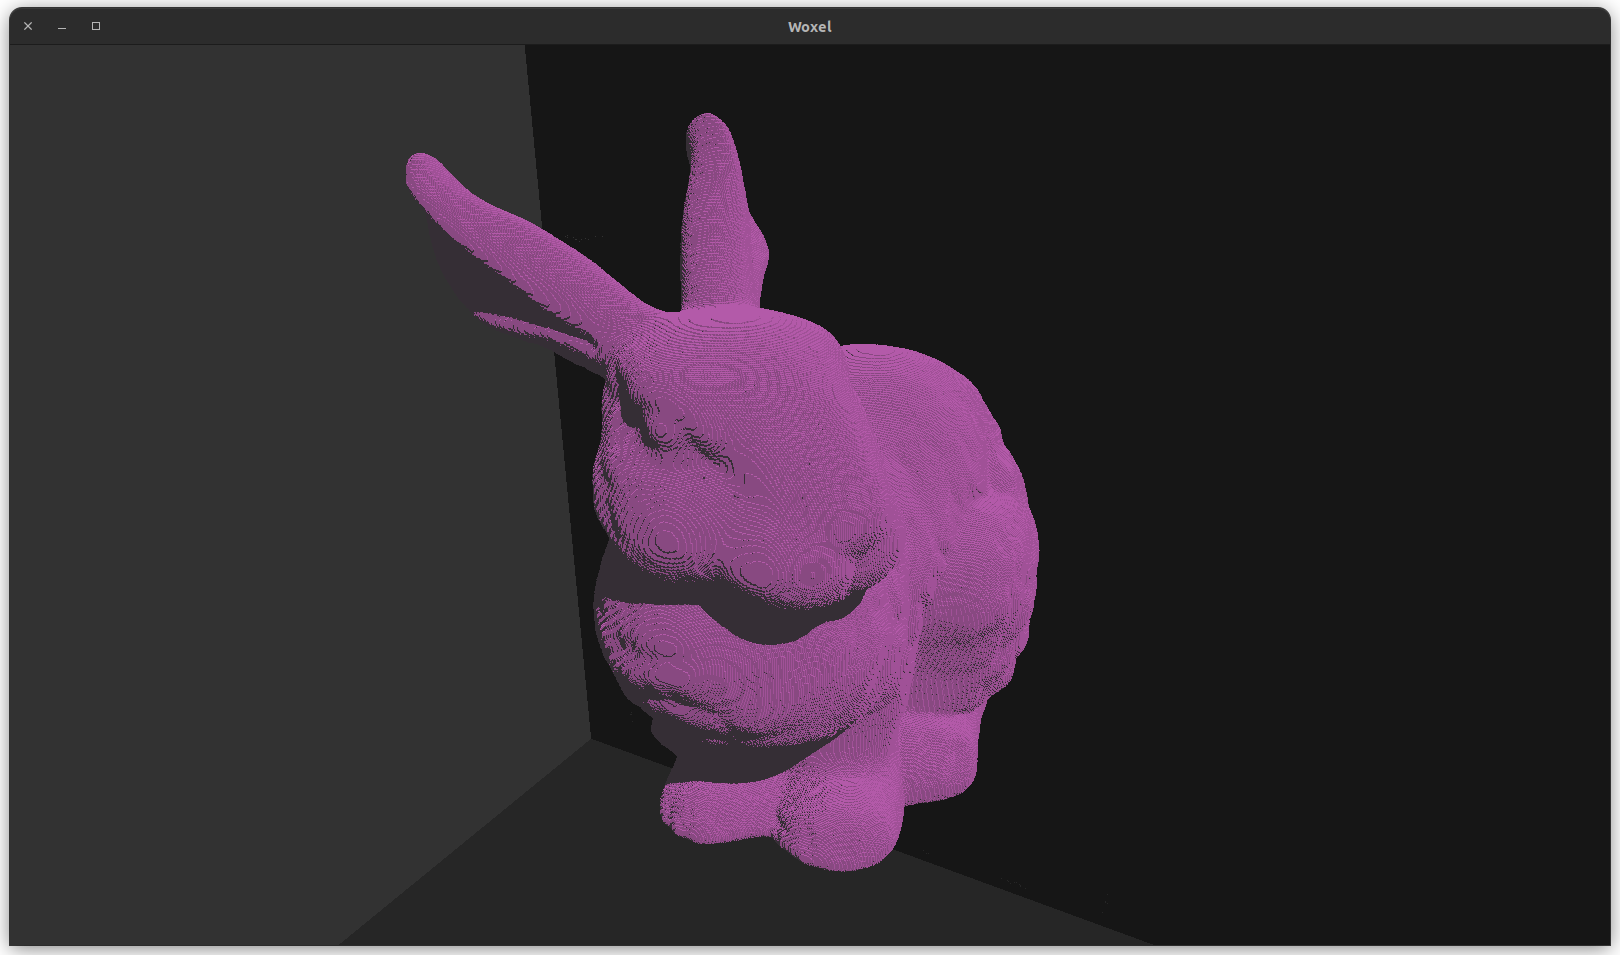
\includegraphics[width=0.8\textwidth]{bunny}
  \caption[Diffuse pink bunny model]{Bunny with diffuse pink material, model voxel resolution: $628\times621\times489$}
\end{figure}

\section{Images}

This section shows some images captured in the rendering engine. All the models used are samples from the OpenVDB website\supercite{openvdb:models}. Each of the figures below showcases the engine's different functionalities.

\begin{figure}[H]
  \centering
  \begin{subfigure}[b]{0.48\textwidth}
    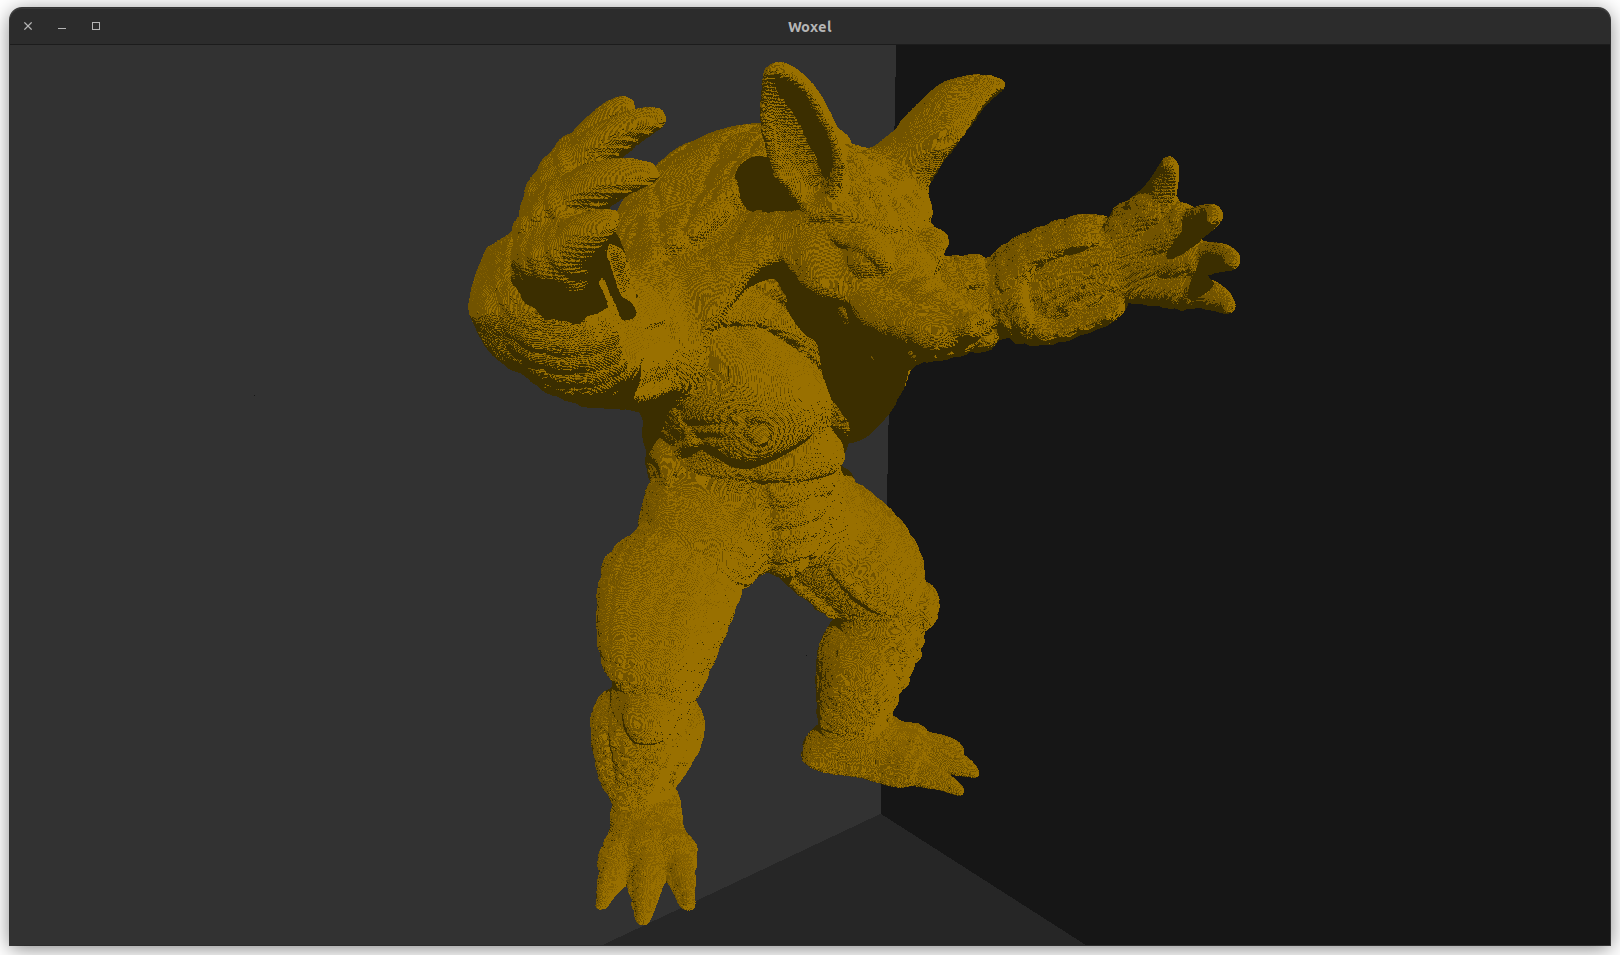
\includegraphics[width=\textwidth]{arm_1}
  \end{subfigure}
  \hfill
  \begin{subfigure}[b]{0.48\textwidth}
    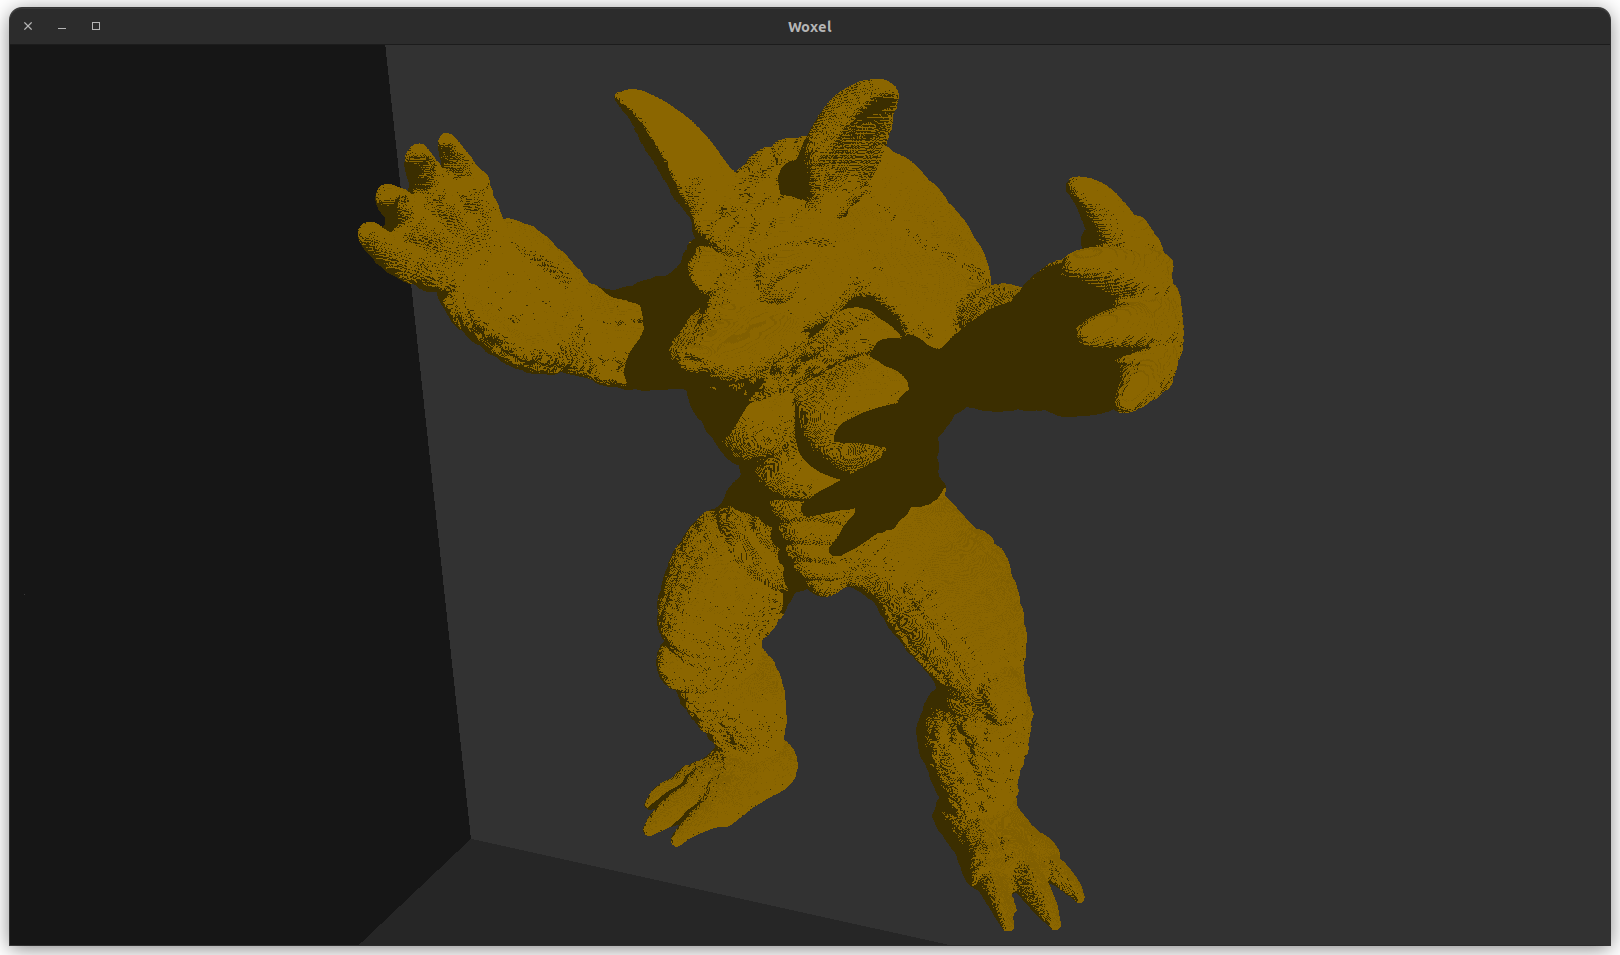
\includegraphics[width=\textwidth]{arm_2}
  \end{subfigure}
  \begin{subfigure}[b]{0.48\textwidth}
    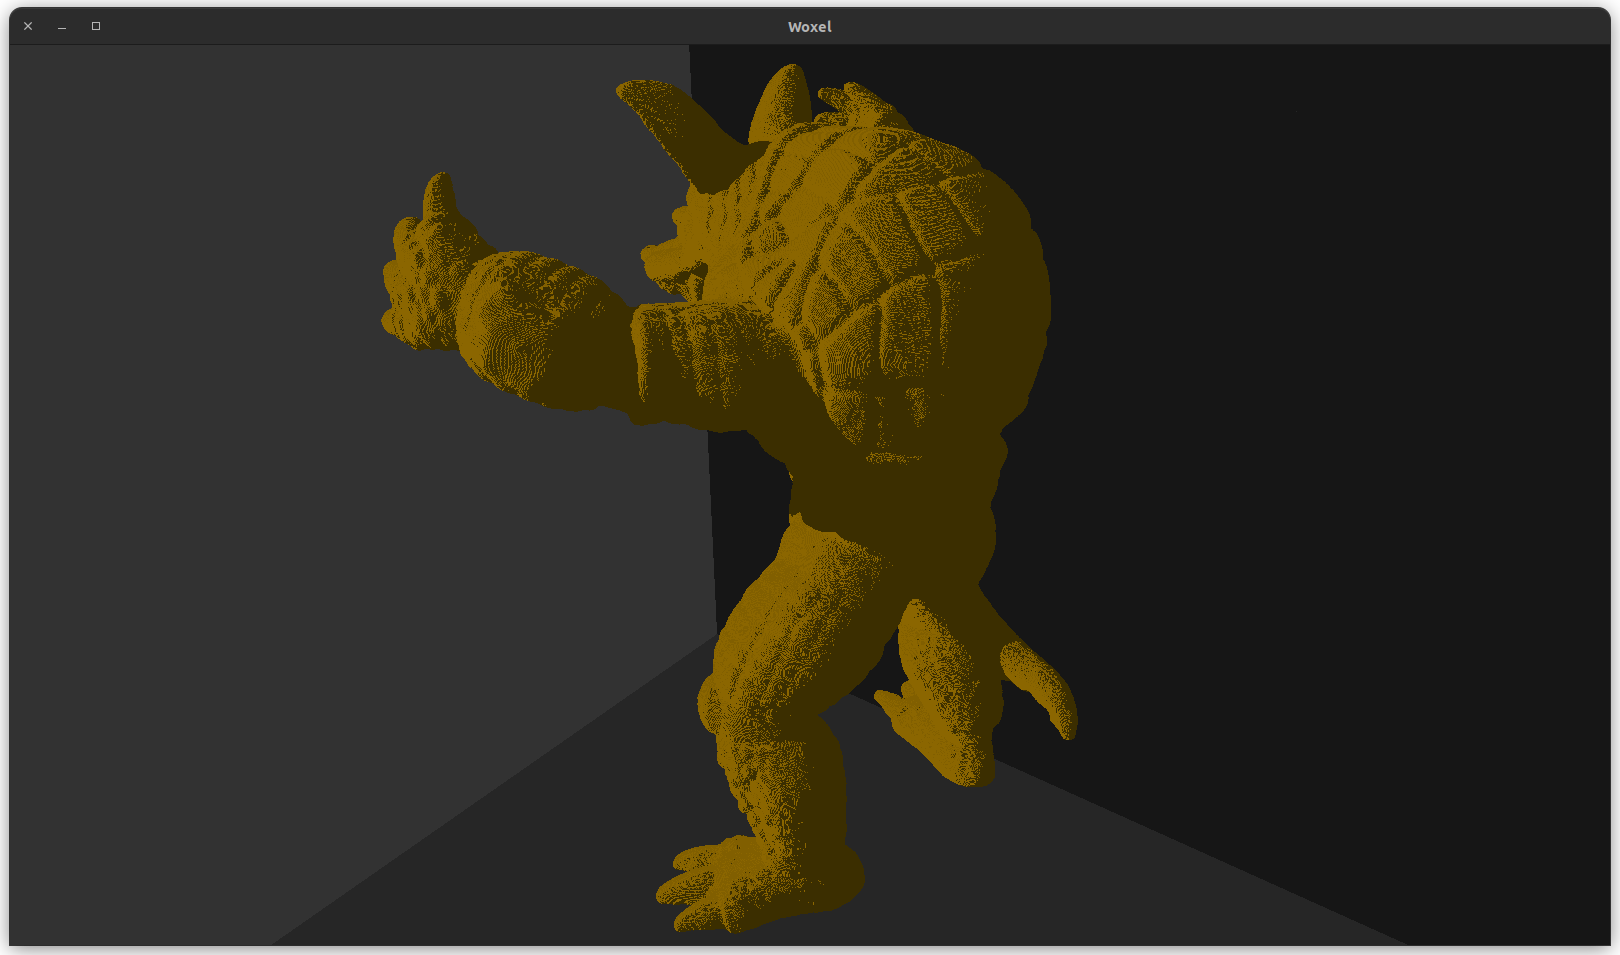
\includegraphics[width=\textwidth]{arm_3}
  \end{subfigure}
  \hfill
  \begin{subfigure}[b]{0.48\textwidth}
    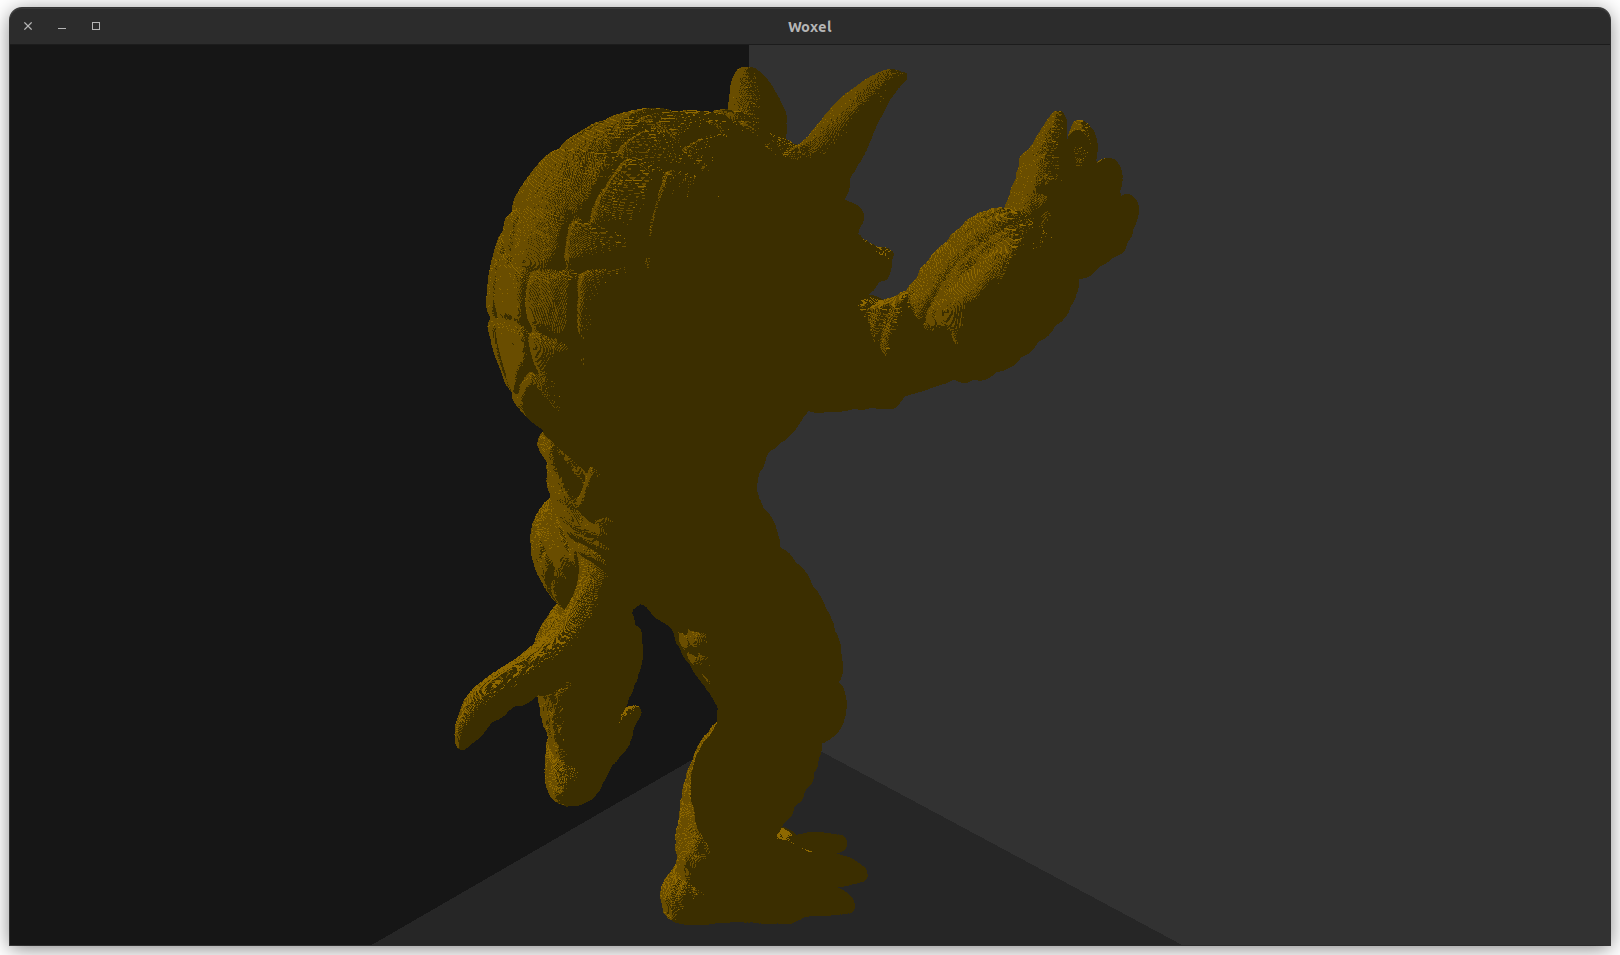
\includegraphics[width=\textwidth]{arm_4}
  \end{subfigure}
  \caption[Armadillo model]{\textbf{Multiple angles} of an armadillo model with a diffuse material. The voxel resolution of the model is $1276\times1518\times116$}
\end{figure}

\newacronym{iss}{ISS}{International Space Station}
\begin{figure}[H]
  \centering
  \begin{subfigure}[b]{0.48\textwidth}
    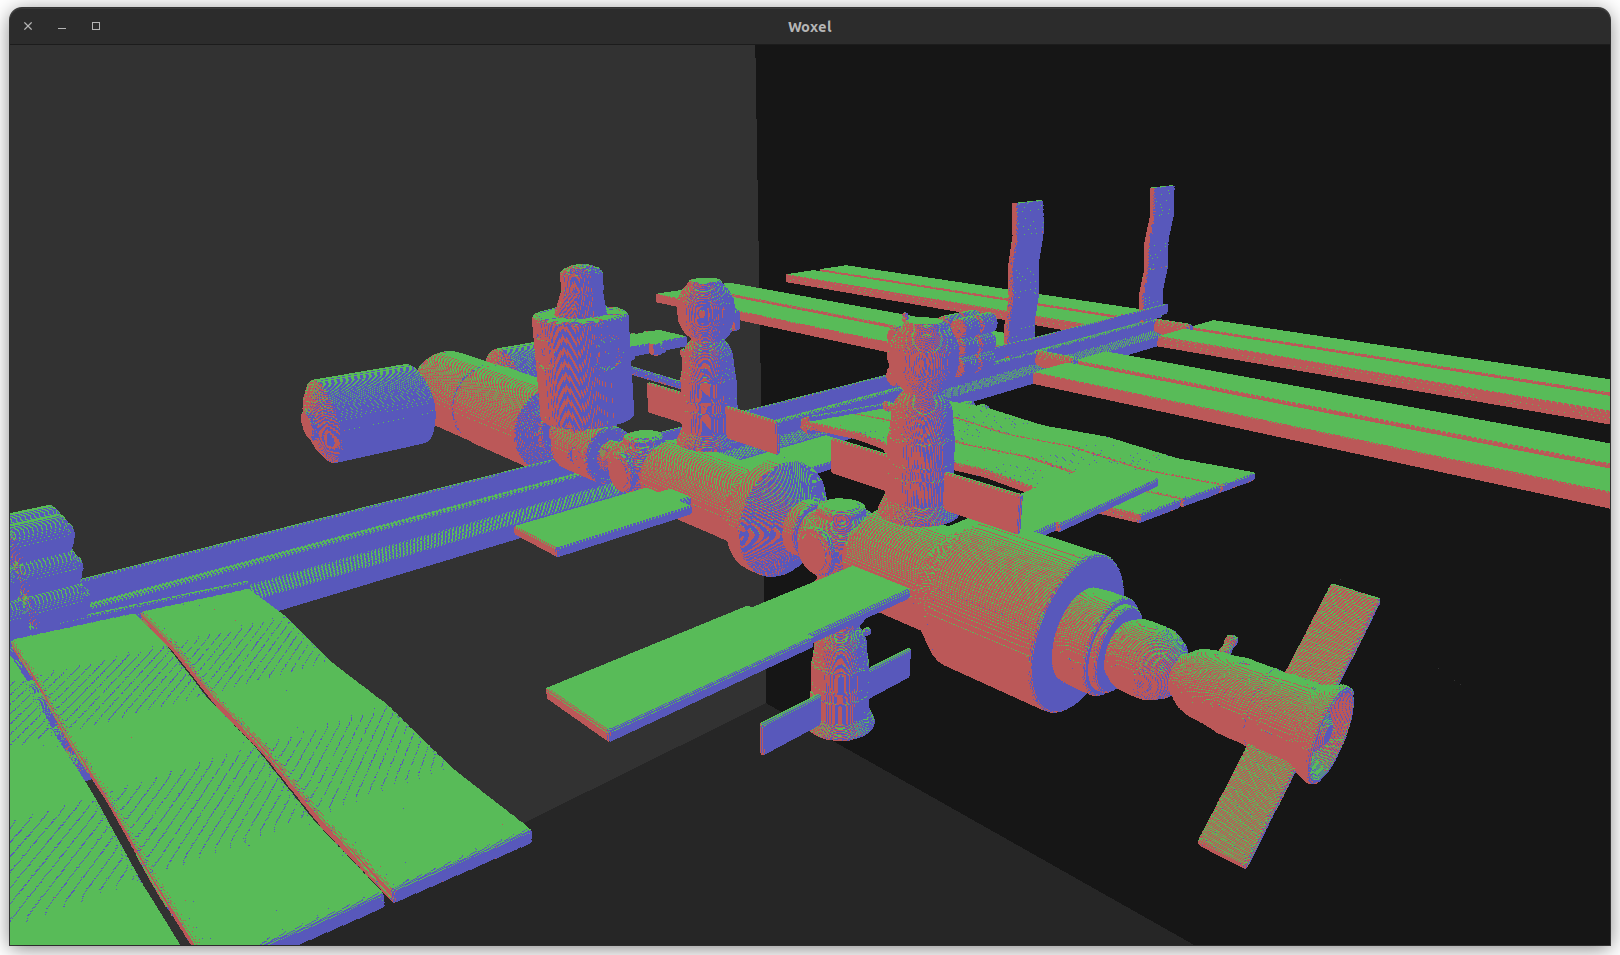
\includegraphics[width=\textwidth]{iss_rgb}
    \caption{RGB}
  \end{subfigure}
  \hfill
  \begin{subfigure}[b]{0.48\textwidth}
    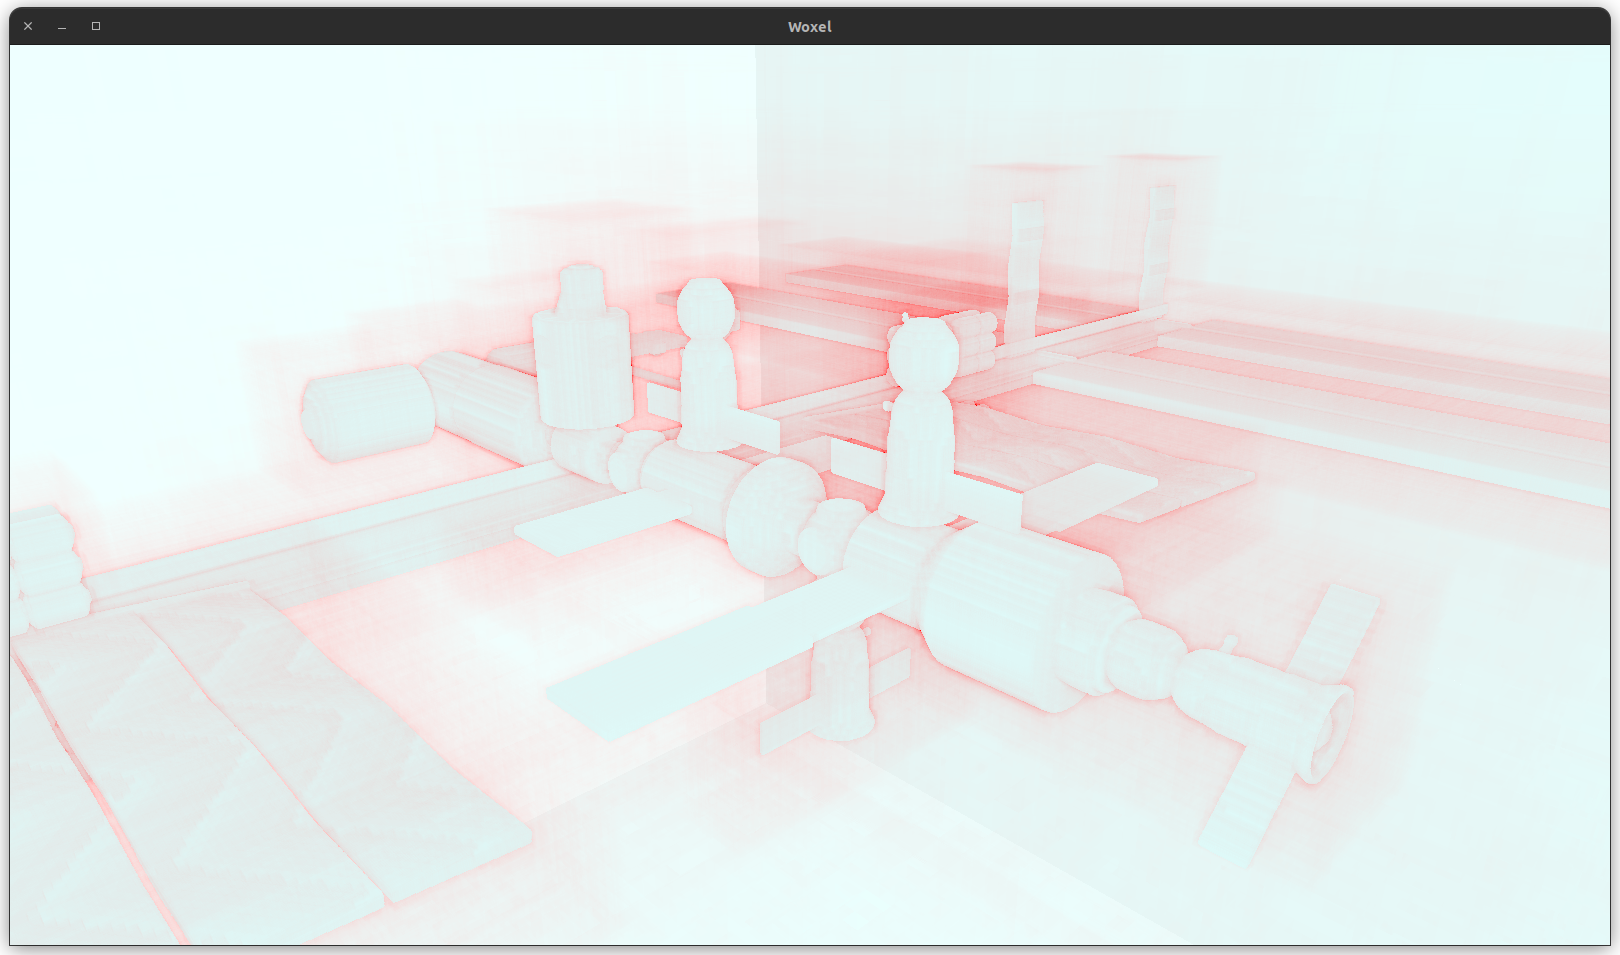
\includegraphics[width=\textwidth]{iss_ray}
    \caption{Ray}
  \end{subfigure}
  \begin{subfigure}[b]{0.48\textwidth}
    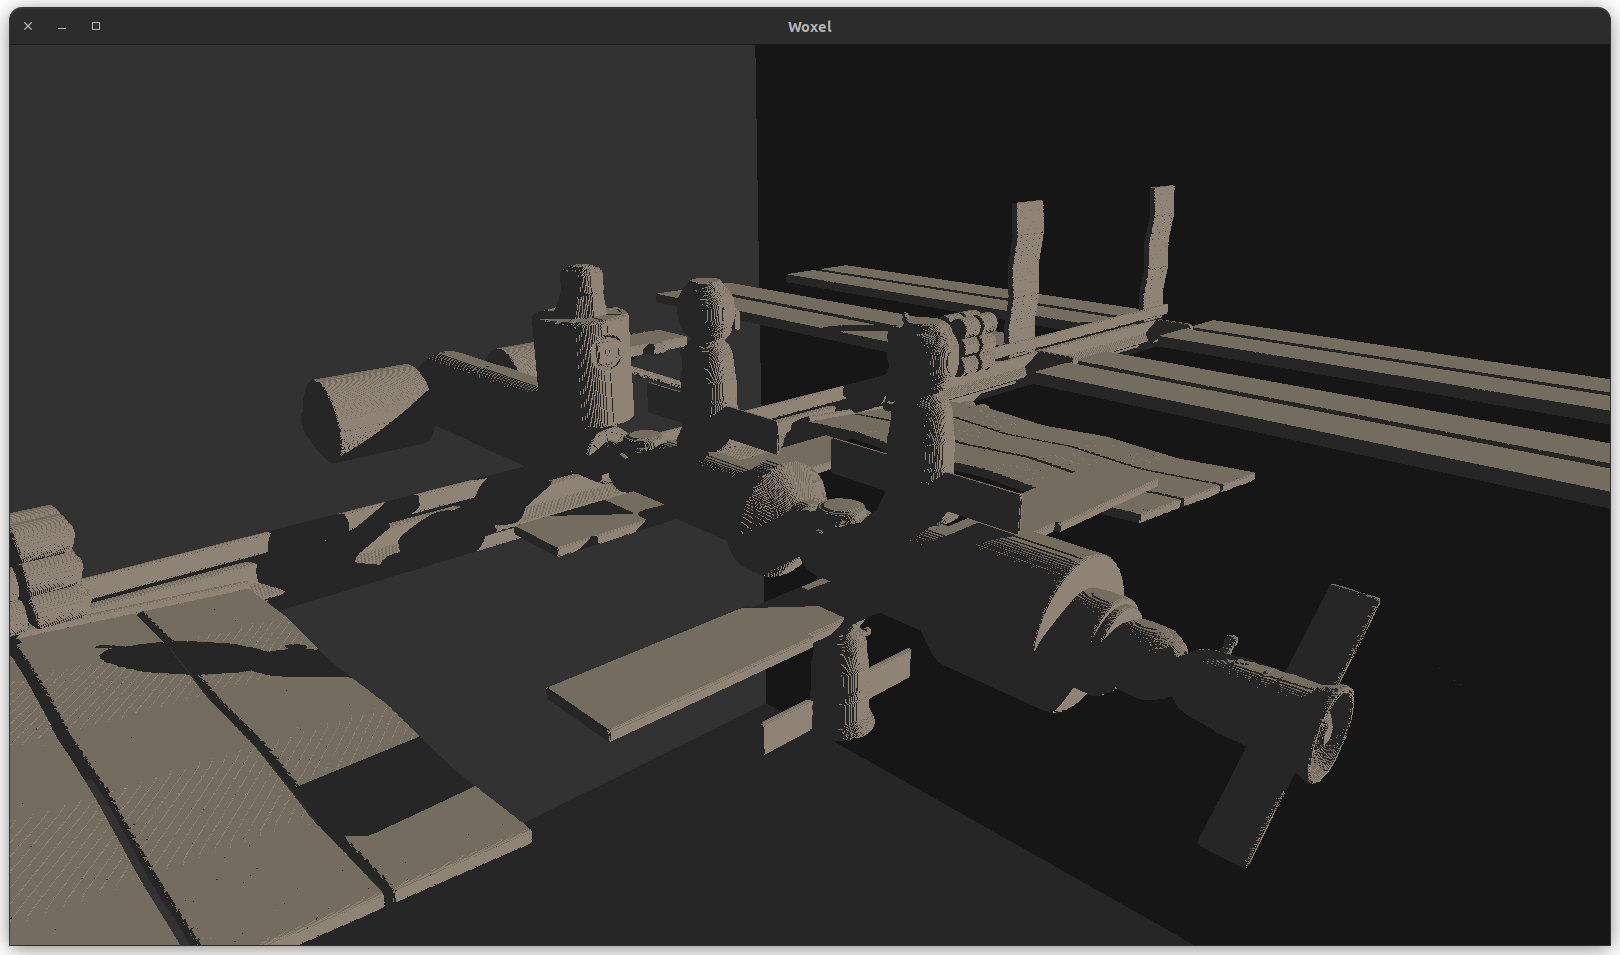
\includegraphics[width=\textwidth]{iss_diffuse}
    \caption{Diffuse}
  \end{subfigure}
  \hfill
  \begin{subfigure}[b]{0.48\textwidth}
    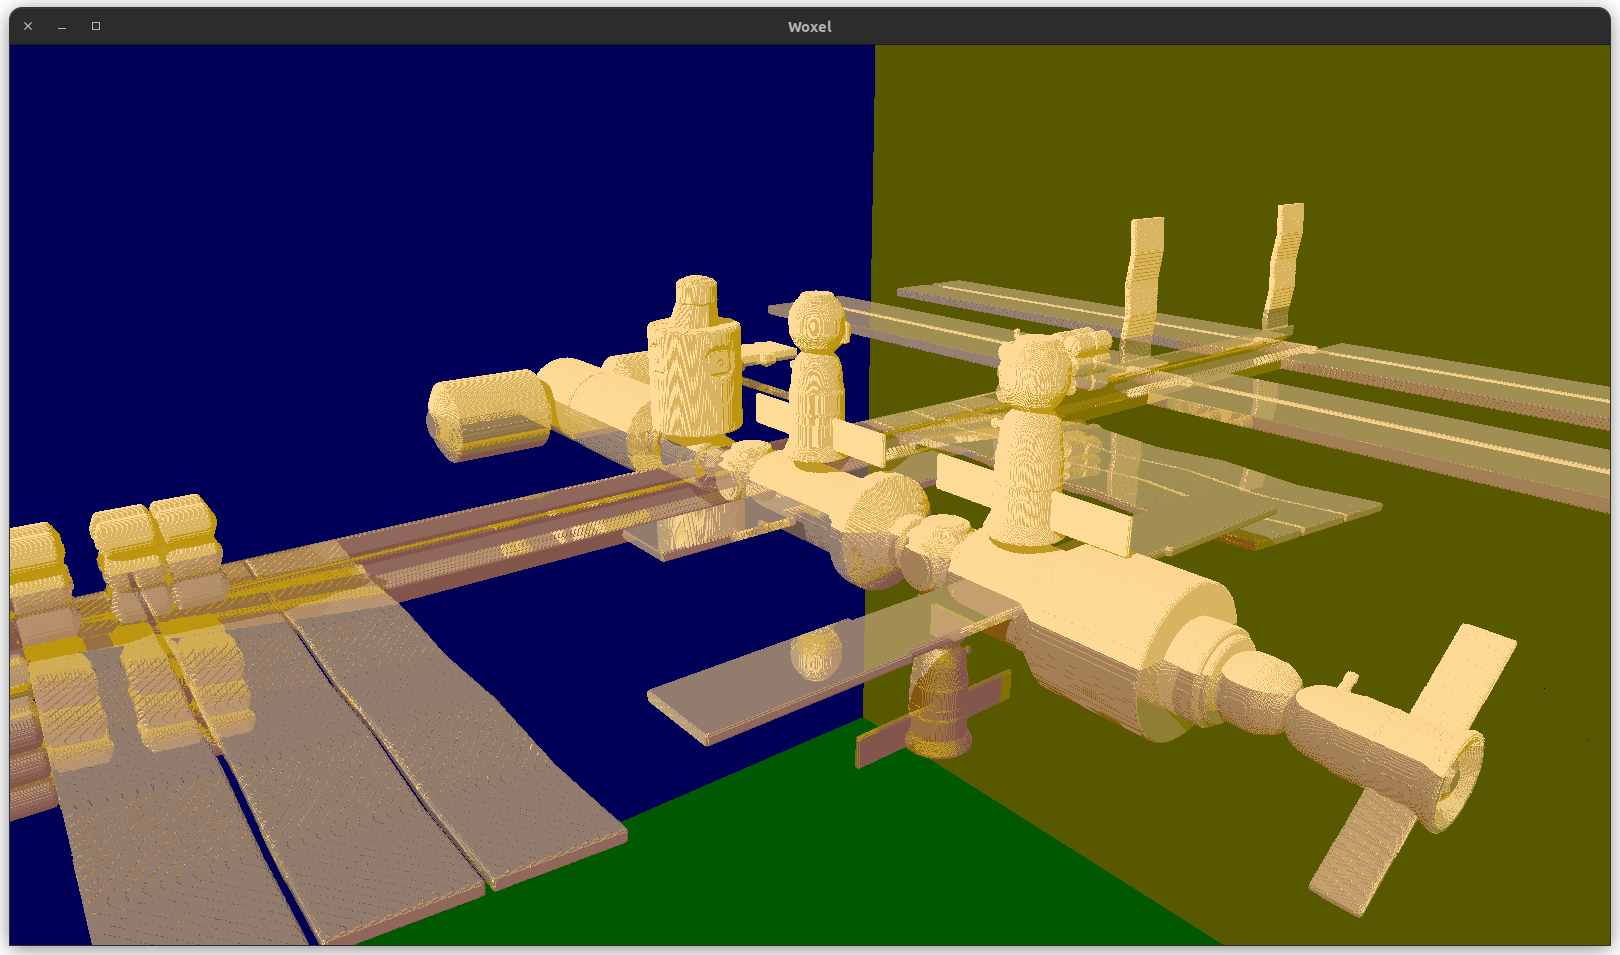
\includegraphics[width=\textwidth]{iss_gloss}
    \caption{Glossy}
  \end{subfigure}
  \caption[ISS model with render modes]{\textbf{Render modes} on a \acrshort{iss} model with voxel resolution $4561\times617\times2999$
    (a): RGB mode colors each face based on the axis to which it is parallel.
    (b): Ray mode colours each pixel based on how many steps the ray took. The colour is interpolated between light blue and red based on how many steps the ray took to go out of bounds or intersect a voxel. The maximum (red) is 200 steps.
    (c): Diffuse mode shows an object with diffuse material lit by sunlight.
    (d): Glossy mode shows a half glossy (bottom), half diffuse (top) model lit by sunlight. The out-of-bounds box is coloured to discriminate which face is reflected on which surface. The reflection of the middle pod with a sphere on top can be seen in the central solar panel. More reflections can be seen in the solar panels on the left and right.
  }
  \label{rendermods}
\end{figure}


\begin{figure}[H]
  \centering
  \begin{subfigure}[b]{0.48\textwidth}
    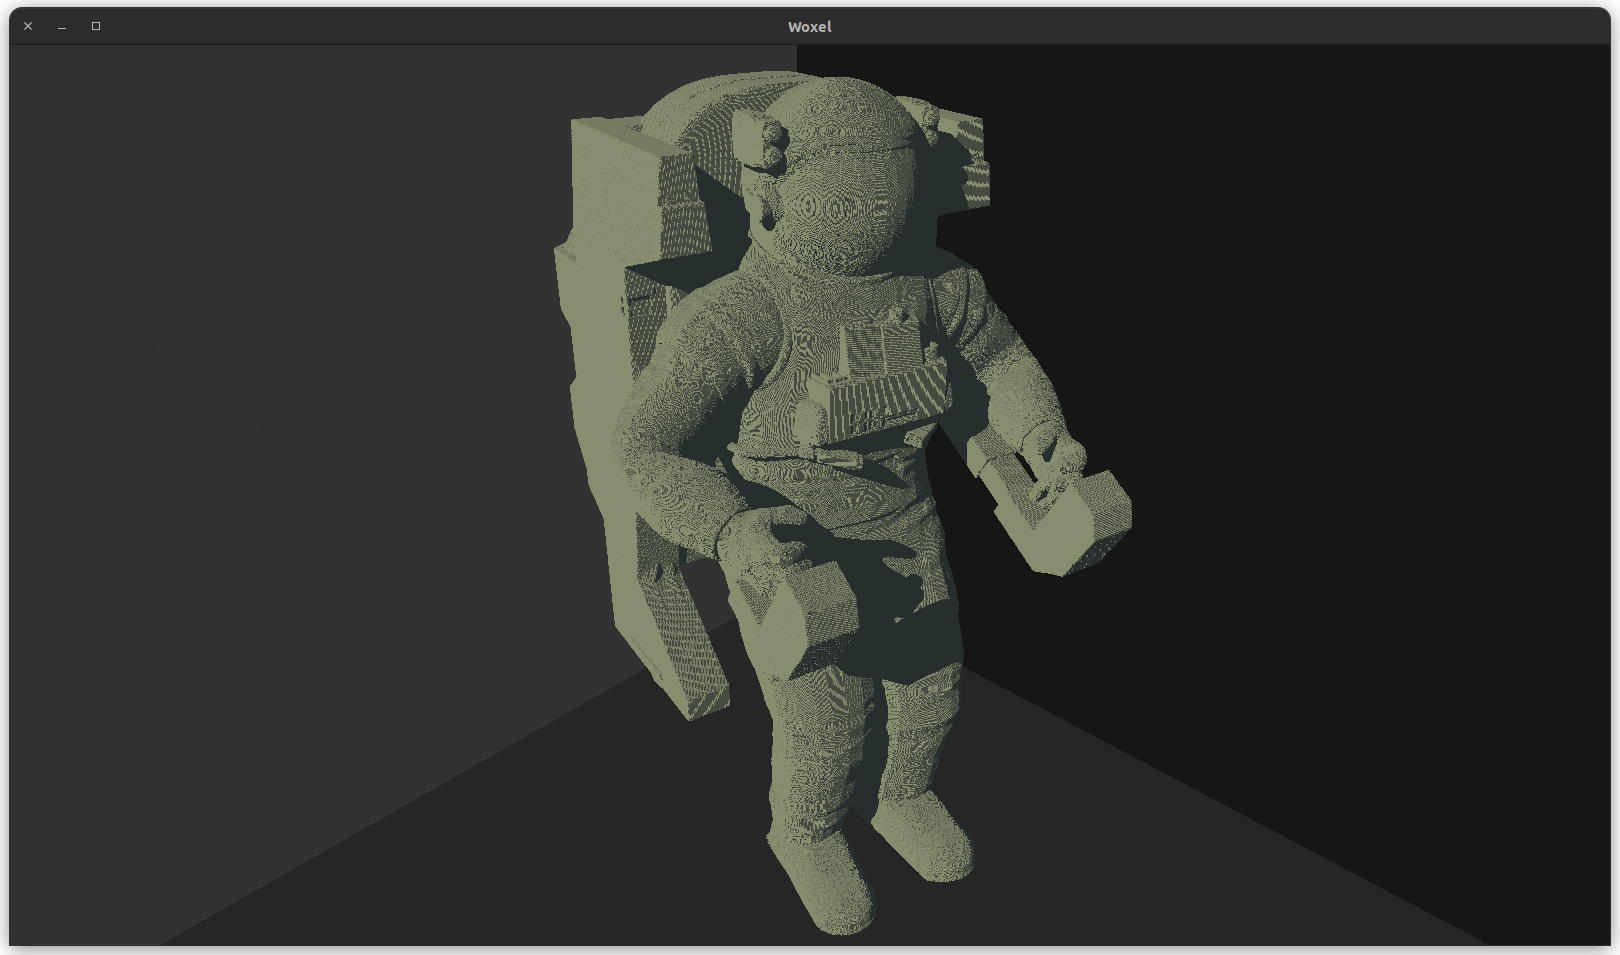
\includegraphics[width=\textwidth]{astro_1}
  \end{subfigure}
  \hfill
  \begin{subfigure}[b]{0.48\textwidth}
    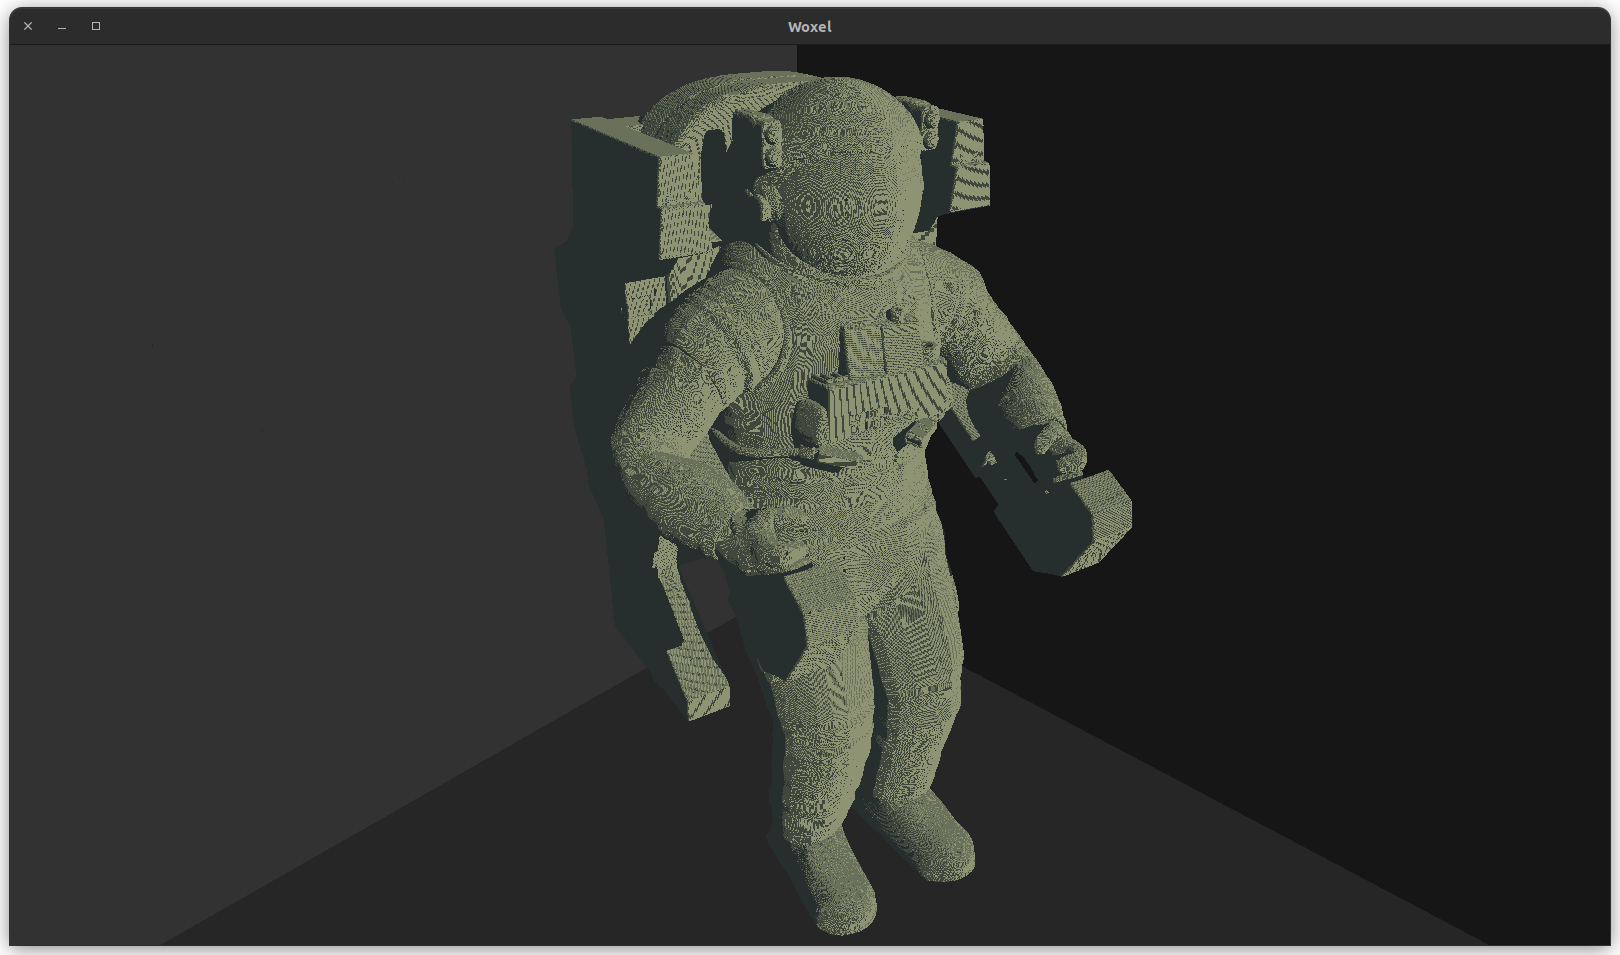
\includegraphics[width=\textwidth]{astro_2}
  \end{subfigure}
  \begin{subfigure}[b]{0.48\textwidth}
    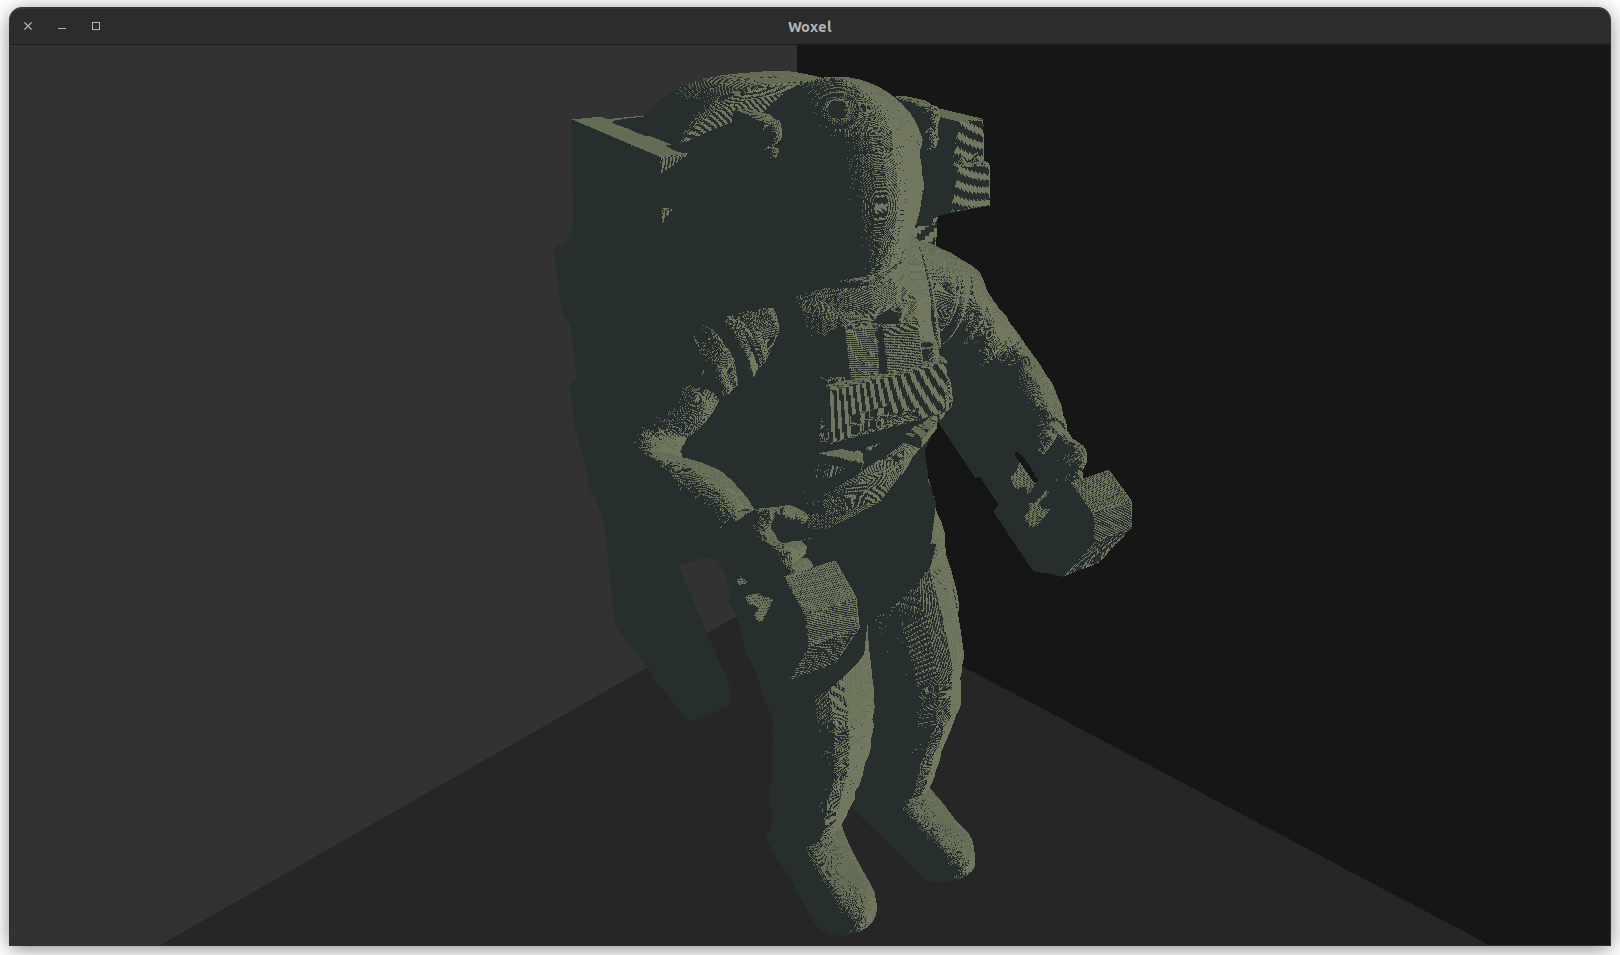
\includegraphics[width=\textwidth]{astro_3}
  \end{subfigure}
  \hfill
  \begin{subfigure}[b]{0.48\textwidth}
    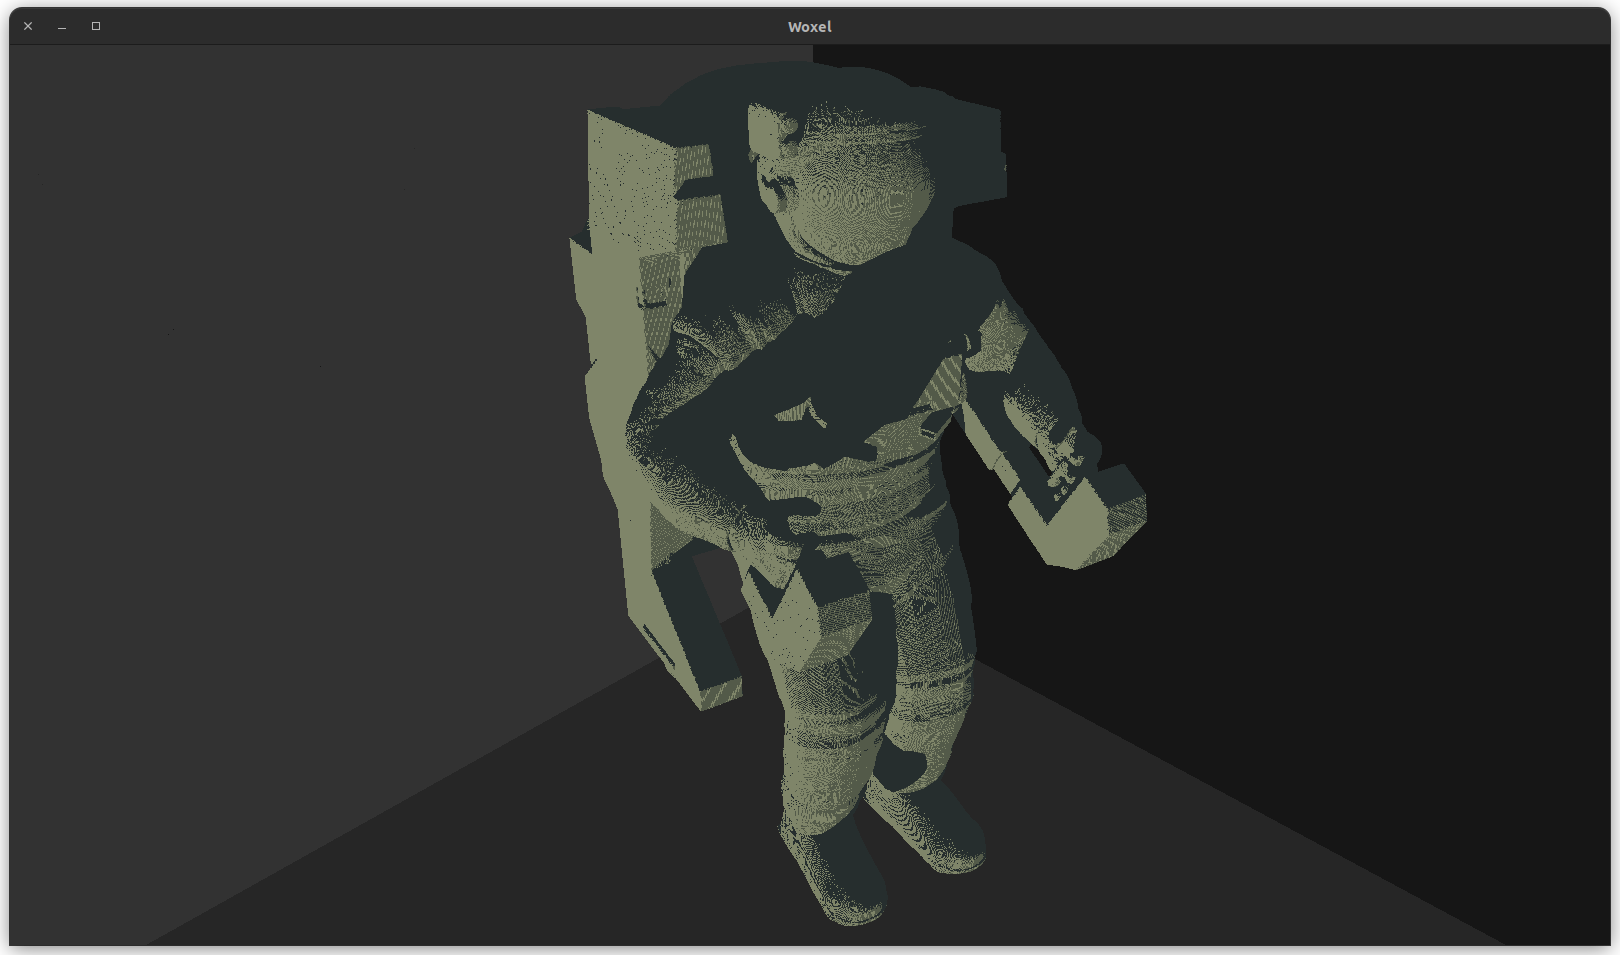
\includegraphics[width=\textwidth]{astro_4}
  \end{subfigure}
  \caption[Astronaut model with dynamic lighting]{\textbf{Dynamic Lighting} on an astronaut model. The sunlight is dynamic; its direction, colour and intensity can be changed through the developer GUI in real time. The voxel resolution of the model is $1481\times2609\times1843$}
\end{figure}

\begin{figure}[H]
  \centering
  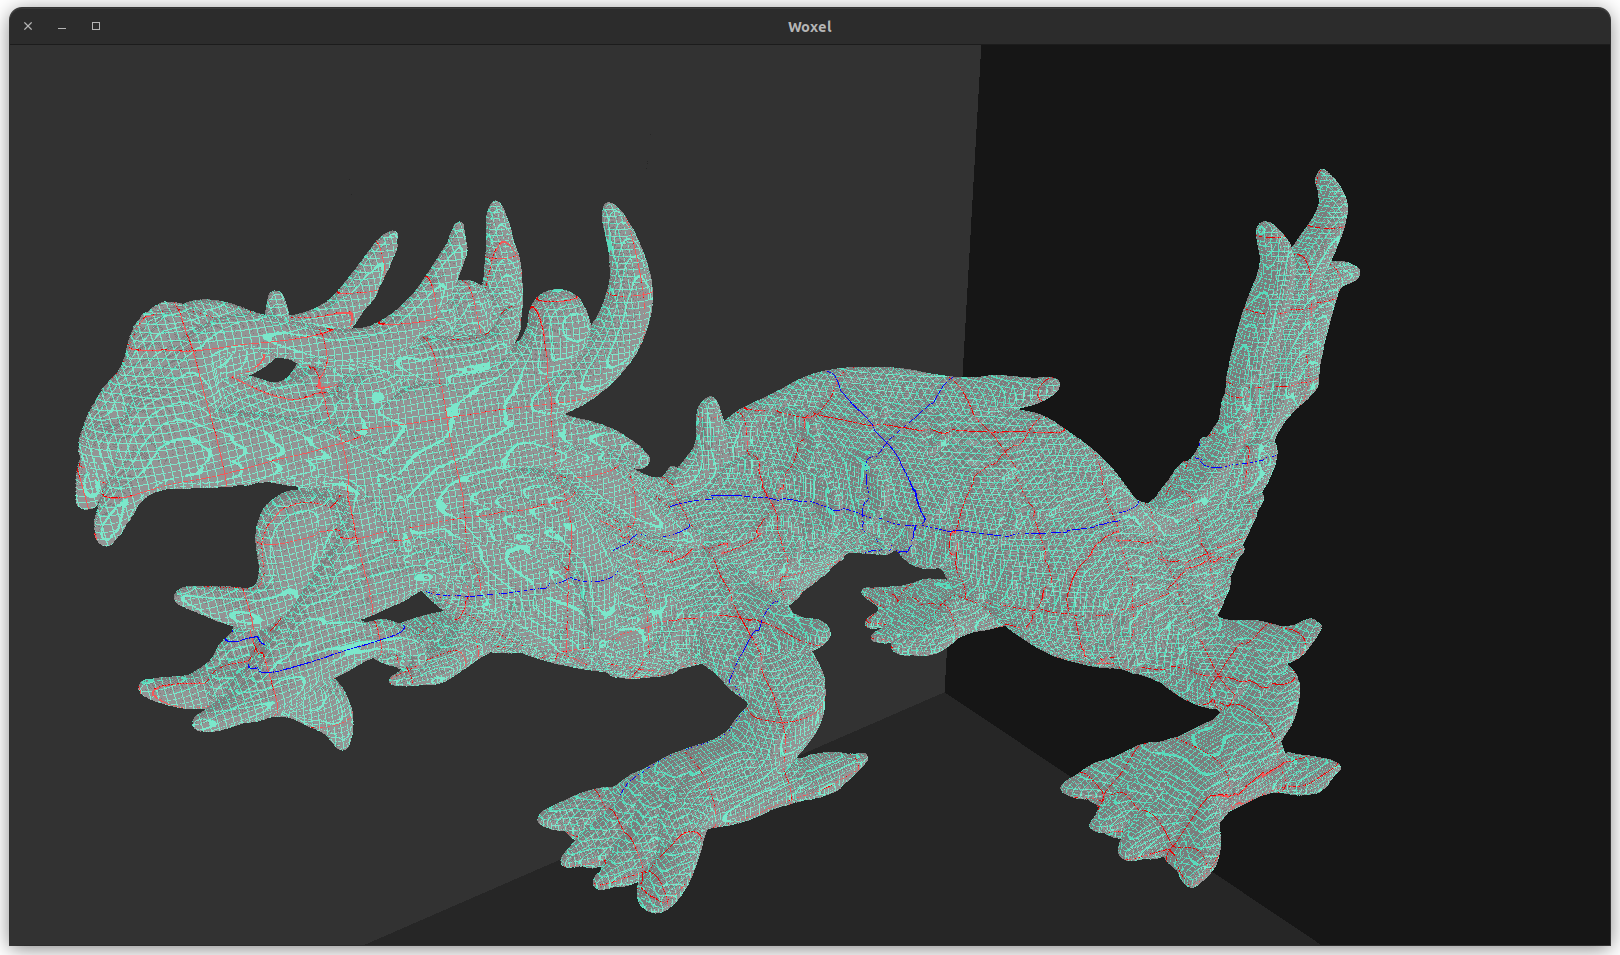
\includegraphics[width=0.8\textwidth]{dragon_3}
  \caption[Dragon model with VDB highlighted]{\textbf{VDB highligthing}: Voxels at the boundaries of VDB nodes are highlighted on a dragon model. The grid structure of the VDB can be seen at each level in the hierarchy. Node3, Node4 and Node5 boundaries are shown in Cyan, Red and Blue, respectively. The voxel resolution of the model is $2023\times911\times1347$}
\end{figure}

\begin{multicols}{2}[]
  \begin{figure}[H]
    \centering
    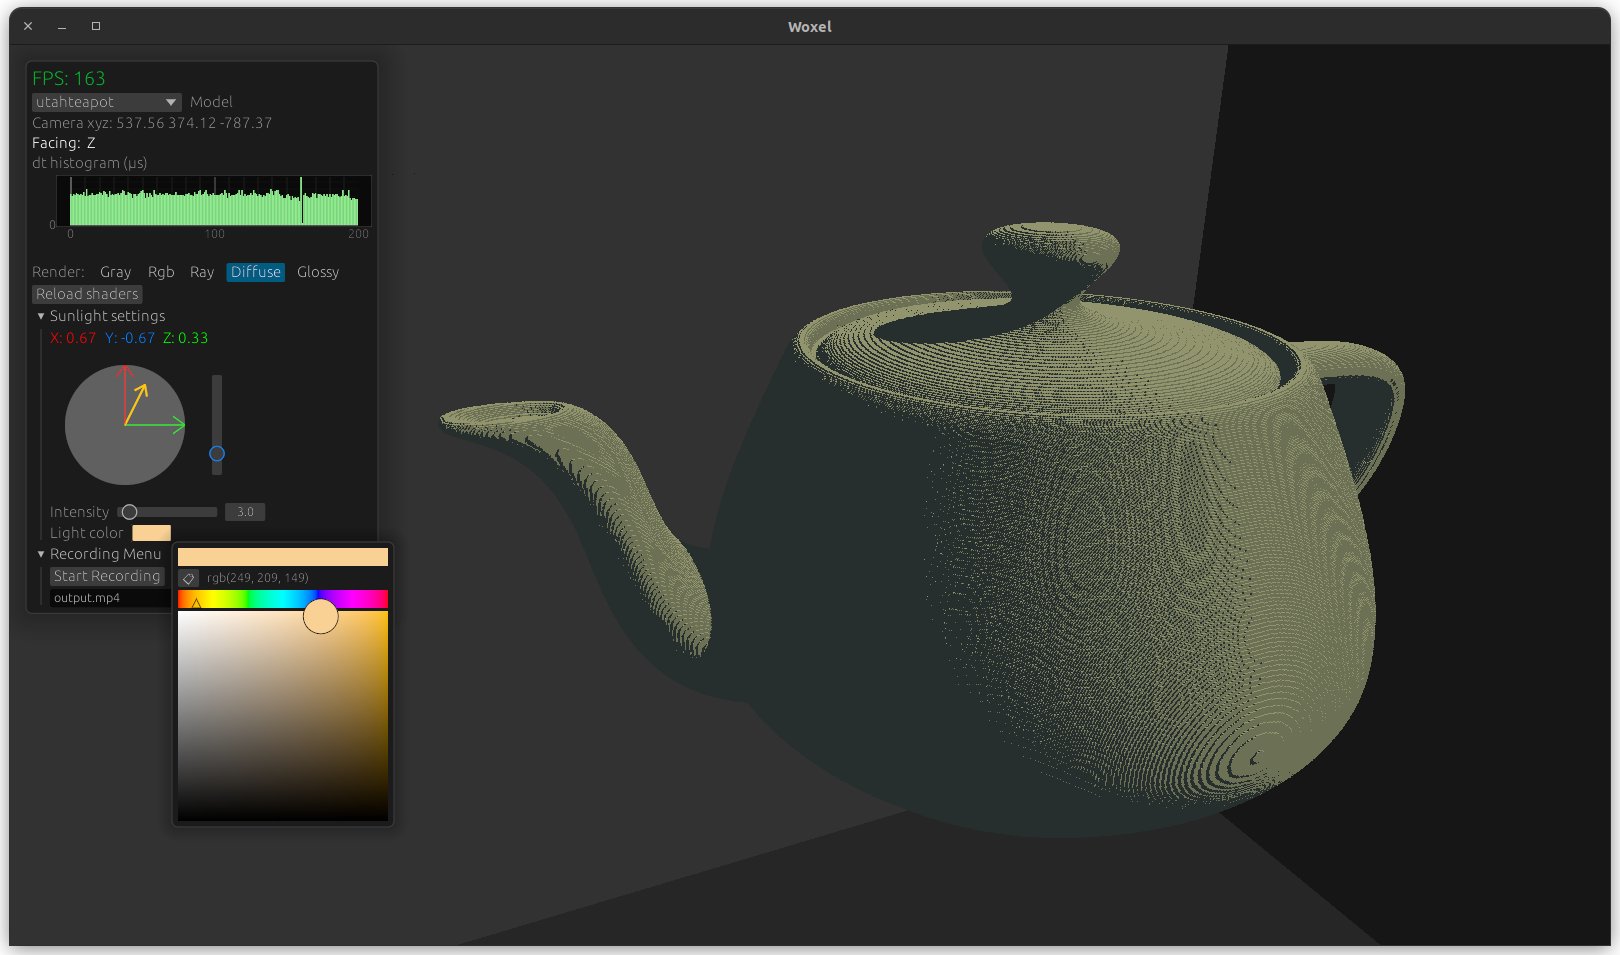
\includegraphics[width=0.96\linewidth]{gui_1}
    \caption[Developer GUI]{Developer GUI in engine}
  \end{figure}
  The developer GUI has the following uses:
  \begin{enumerate}[itemstep=0mm]
    \item Display current \acrshort{fps} and histogram of milliseconds per frame.
    \item Changing the model in the viewport through a drop-down menu that scans the assets folder for available models.
    \item Camera coordinates and facing direction
    \item Functionality to change between the render modes presented in \cref{rendermods}
    \item The option to reload the shaders while the engine is running.
    \item There is a sunlight section available for the diffuse and glossy render modes.
    \item The recording menu allows setting an output file and starting or ending the recording.
  \end{enumerate}
  \columnbreak
  \begin{figure}[H]
    \centering
    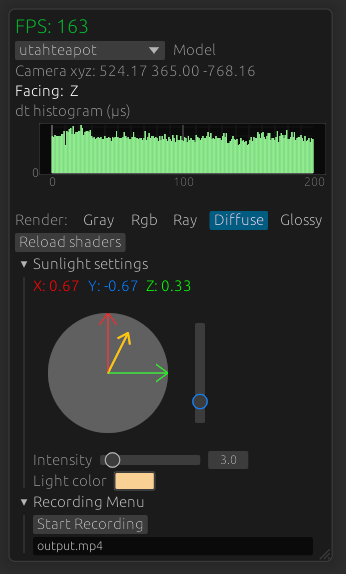
\includegraphics[width=1.0\linewidth]{gui_2}
    \caption{Developer GUI close-up}
    \label{gui}
  \end{figure}
\end{multicols}

\section{Experiments}
This section compares the ray casting algorithms against each other on different models and render modes.

The specifications of the machine the experiments were run on are presented in \cref{specs}.
\begin{table}[h]
  \centering
\begin{tabular}{|c||c|}
  \hline
  \multicolumn{2}{|c|}{Experiment machine specifications} \\
  \hline
  OS & Ubuntu 22.04.3 LTS x86\_64\\
  \hline
  CPU & AMD Ryzen 7 5800H with Radeon\\
  \hline
  GPU &  NVIDIA GeForce RTX 3070 Mobile\\
  \hline
  RAM & 8192MiB \\
  \hline
  FMA & Enabled \\
  \hline
\end{tabular}
  \caption{Experiment machine specifications}
  \label{specs}
\end{table}

\subsection{Comparing DDA, HDDA and HDDA+SDF}

The average milliseconds per frame are compared for the DDA, HDDA and HDDA+SDF algorithms on the teapot model (voxel resolution of $981\times462\times617$) on the ray render mode at three distinct distances from the model, one further away or closer and one near the model. Checking at three separate distances is essential because the performance of the hierarchical algorithms depends on the topology the camera rays are going through. When the target object is far away, most camera rays can traverse the VDB at higher levels in the tree since there is no detail around them. Conversely, when the camera is closer to the object, the rays must traverse more complex topology at lower levels in the tree, and therefore the algorithm can be slower.

\begin{table}[h]
  \centering
  \begin{tabular}{|c||c|c|c|}
    \hline
    & 2000m & 1000m & 500m \\
    \hline
    DDA & 100.3ms* & 100.1ms* & 50.4ms \\
    \hline
    HDDA & 9.4ms & 12.5ms & 14.4ms \\
    \hline
    HDDA+SDF & 6ms** & 6.4ms & 7.6ms\\
    \hline
  \end{tabular}
  \caption[DDA vs. HDDA vs. HDDA+SDF on teapot model]{Milliseconds per frame of rendering the teapot model using DDA, HDDA, HDDA+SDF at far, medium, and close distances. A voxel is considered $1\rm{m}\times1\rm{m}\times1\rm{m}$. The average ms per frame is taken from a 1000 frame interval.\\
    *: The model does not appear in the viewport because the algorithm exceeds the maximum step count of 1000. This time can be treated as the worst-case, casting bouncing the maximum number of times for each pixel.\\
    **: Frame rate cap is hit at 165 FPS; this is as good as the ray casting can get on this machine}
  \label{table:2}
\end{table}

\begin{figure}[H]
  \centering
  \begin{subfigure}[b]{0.48\textwidth}
    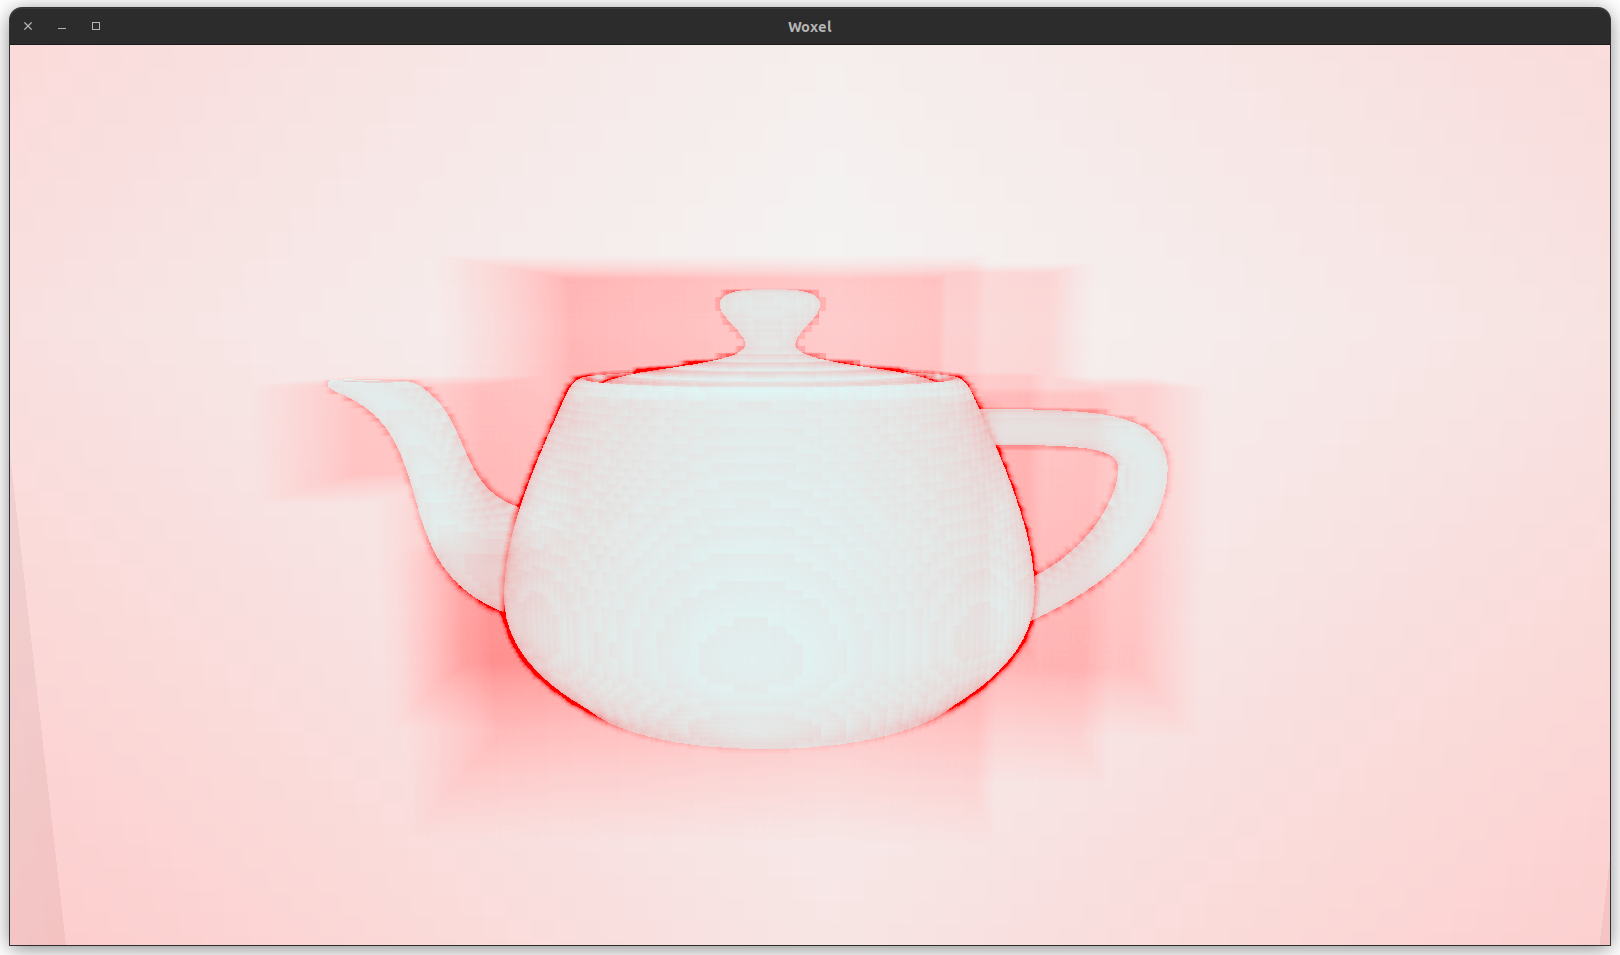
\includegraphics[width=\textwidth]{teapot_2}
    \caption{}
  \end{subfigure}
  \hfill
  \begin{subfigure}[b]{0.48\textwidth}
    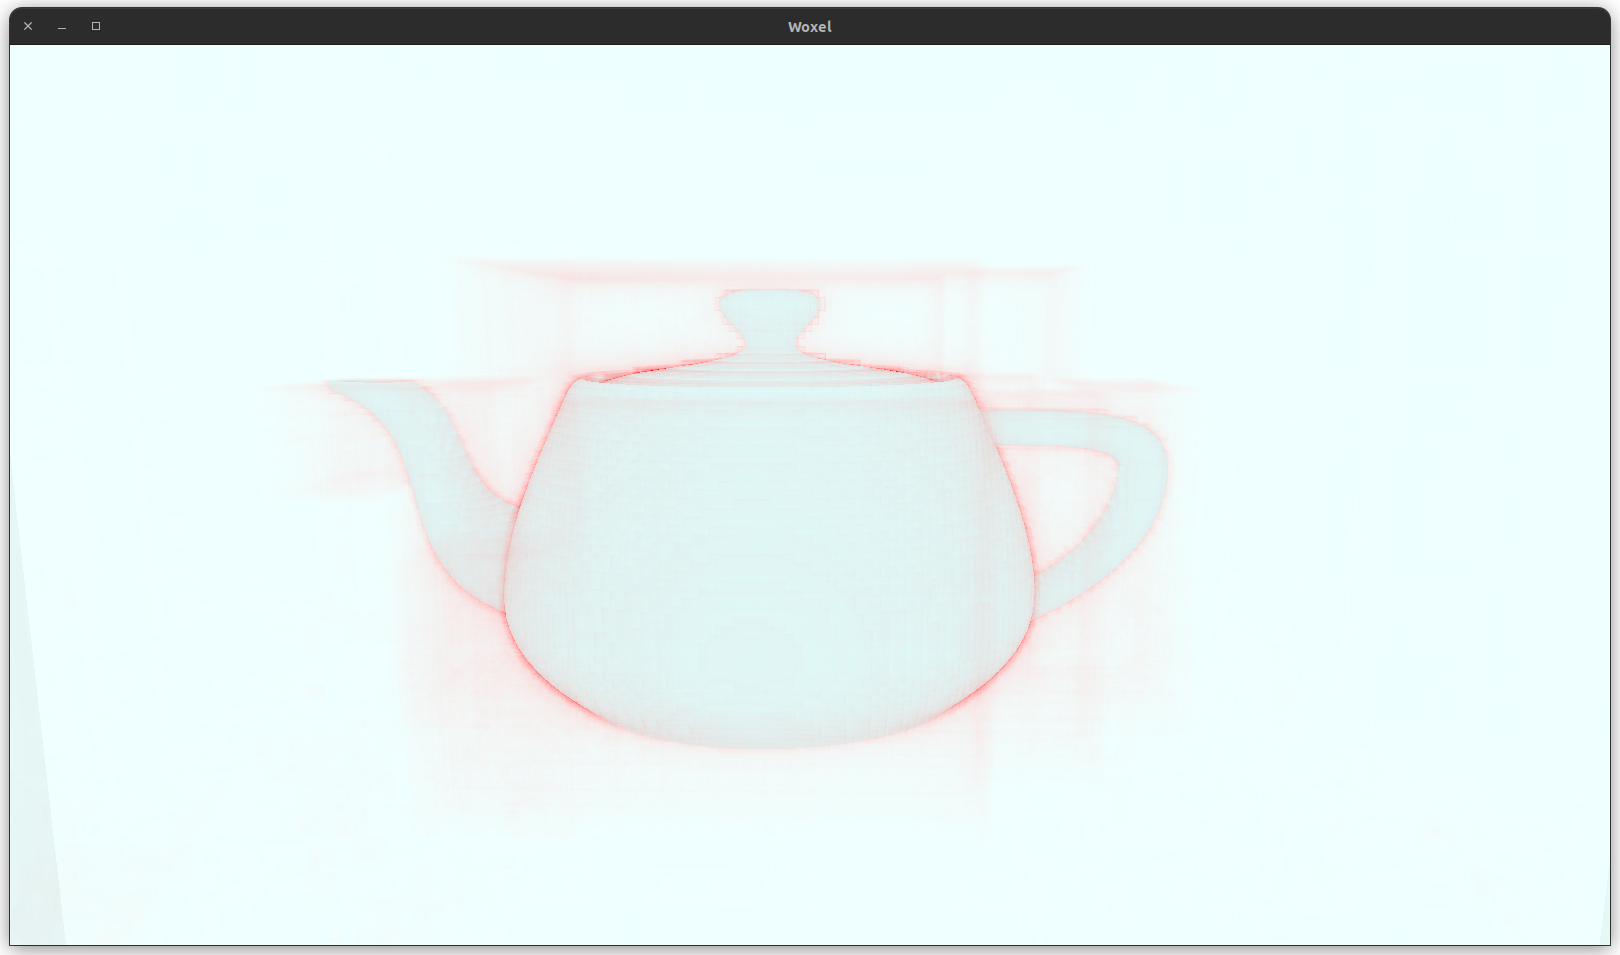
\includegraphics[width=\textwidth]{teapot_1}
    \caption{}
  \end{subfigure}
  \caption[Teapot HDDA vs. HDDA+SDF comparison]{Render in ray mode using (a) HDDA and (b) HDDA+SDF on the teapot model from a 1000m distance. The model resolution is $981\times462\times617$. As in \cref{rendermods}(b), the colour of pixels is determined based on the steps the ray took to intersect the model. The maximum is 200 steps, which corresponds to bright red.}
  \label{teacomp}
\end{figure}

The DDA version cannot handle a mesh of this resolution since rays are marched one voxel at a time. At 2000 voxels away, no ray can reach the object before it exceeds the maximum step count of 1000. At 500 voxels away, the DDA manages to render part of the teapot at 50 milliseconds per frame ($20$ FPS), which is not enough for modern engines.
Both the HDDA and HDDA+SDF perform very well on this model. The HDDA algorithm has a minimum FPS of 70 at the 500m point. The HDDA+SDF manages to hit the GPU's frame rate cap at 165 FPS at the 2000m point and does not drop below 120 FPS at the close point. Adding the SDF to the HDDA algorithm yields a performance boost of $36\%$ at 2000m, $49\%$ at 1000m, and $47\%$ at 500m.

It is visible in \cref{teacomp} that most of the improvement the SDF offers is for pixels whose corresponding camera rays don't intersect voxels. This is because voxels are intersected relatively quickly in the classic HDDA. The slowest raycasting operations are those that pass voxels very close by and go then off into the background, as shown in \cref{steps}. This is precisely where the SDF is most valuable since it can get the ray out of those high-detail areas faster. Moreover, when the ray travels in low detail space, there is also an improvement because the further the ray gets from the object, the further it will step. This allows rays to get out of bounds much faster.

\begin{figure}[H]
  \centering
  \begin{subfigure}{0.45\textwidth}
    \centering
    \includesvg[width=\textwidth]{steps.svg}
    \caption{}
  \end{subfigure}
  \begin{subfigure}{0.45\textwidth}
    \centering
    \includesvg[width=\textwidth]{steps_sdf.svg}
    \caption{}
  \end{subfigure}
  \caption[HDDA vs. HDDA+SDF near-miss diagram]{ray that intersects voxel vs. ray that ``near-misses'' it. (a) HDDA algorithm; the first has 2 axis crossings, the latter has 9 (b) HDDA+SDF algorithm; the first has 2 axis crossings, the latter has 6.}
  \label{steps}
\end{figure}

The same experiment setup is repeated for the ISS model because it has many gaps and tight spaces in its geometry. This time, only HDDA and HDDA+SDF are considered since the DDA could not handle the teapot model, which is much smaller than the ISS. Another change is that the camera positions used are no longer based on the distance to the object but instead positioned such that increasing levels of detail and overlapping geometry are in view.

\begin{table}[h]
  \centering
  \begin{tabular}{|c||c|c|c|}
    \hline
    & pos. 1 & pos. 2 & pos. 3 \\
    \hline
    HDDA & 9.1ms & 10.6ms & 15.3ms \\
    \hline
    HDDA+SDF & 6ms** & 7.2ms & 8.3ms\\
    \hline
    improvement & 36\% & 32\% & 46\%\\
    \hline
  \end{tabular}
  \caption[HDDA vs. HDDA+SDF on ISS model]{Milliseconds per frame of rendering the \acrshort{iss} model using HDDA, HDDA+SDF at three positions in space selected to be increasingly detailed. The average ms per frame is taken from a 1000 frame interval. The improvement from HDDA to HDDA+SDF is also recorded. \\
    **: Frame rate cap is hit at 165 FPS; this is as good as the ray casting can get on this machine}
\end{table}

\begin{figure}[H]
  \centering:
  \begin{subfigure}[b]{0.45\textwidth}
    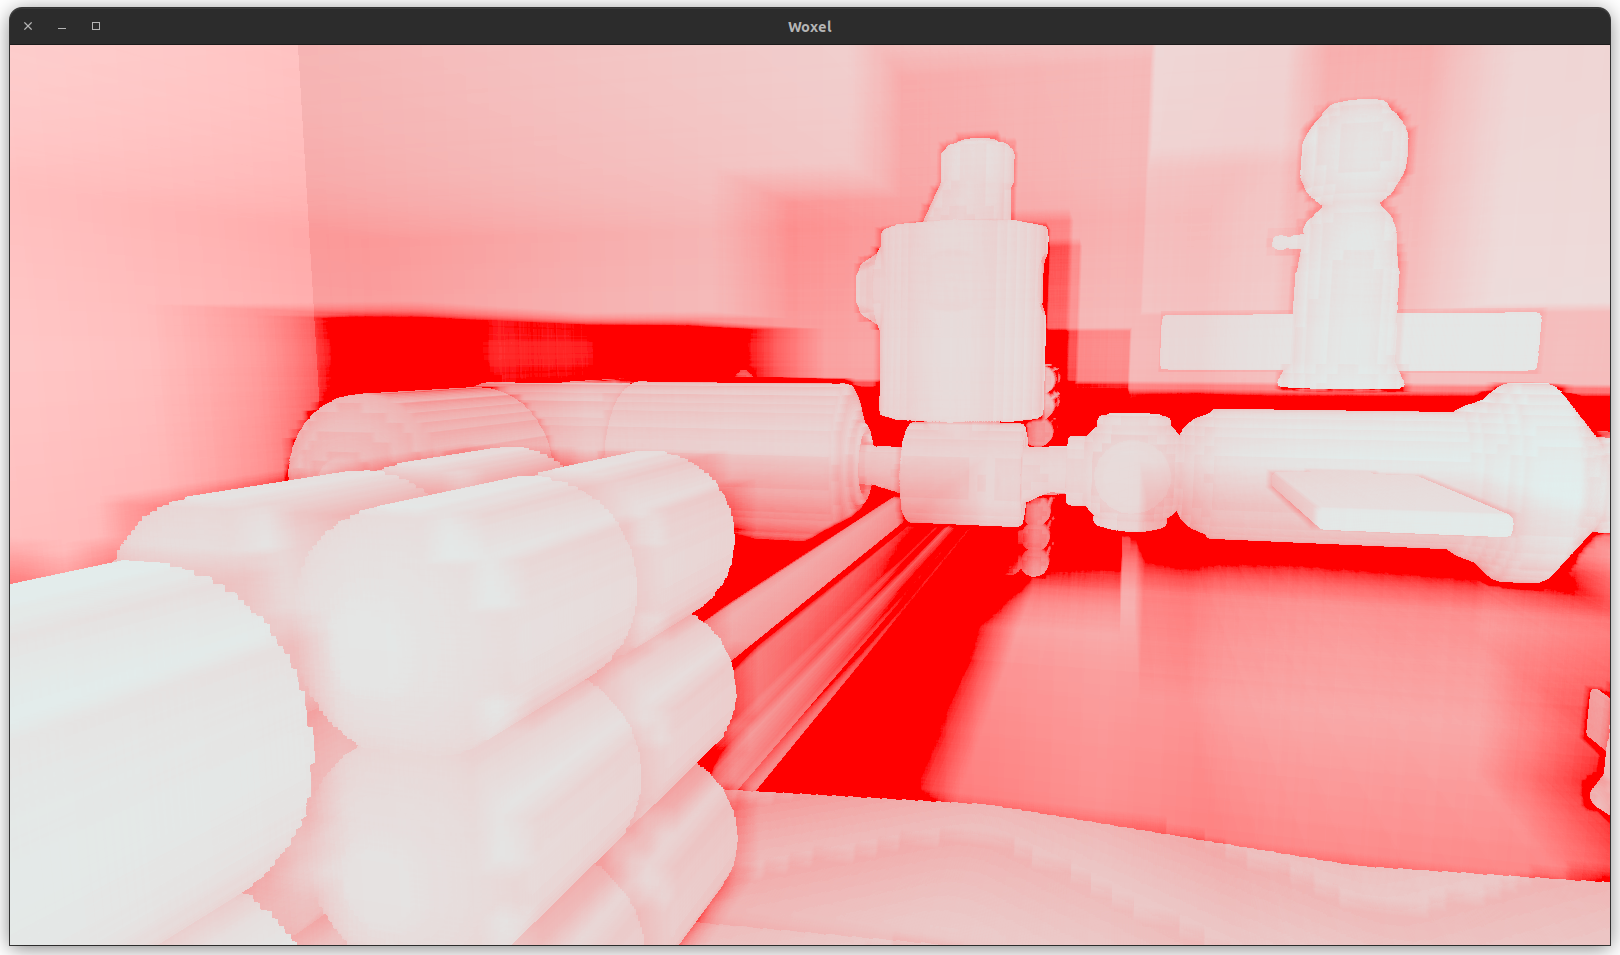
\includegraphics[width=\textwidth]{iss_hdda}
    \caption{}
  \end{subfigure}
  \hfill
  \begin{subfigure}[b]{0.45\textwidth}
    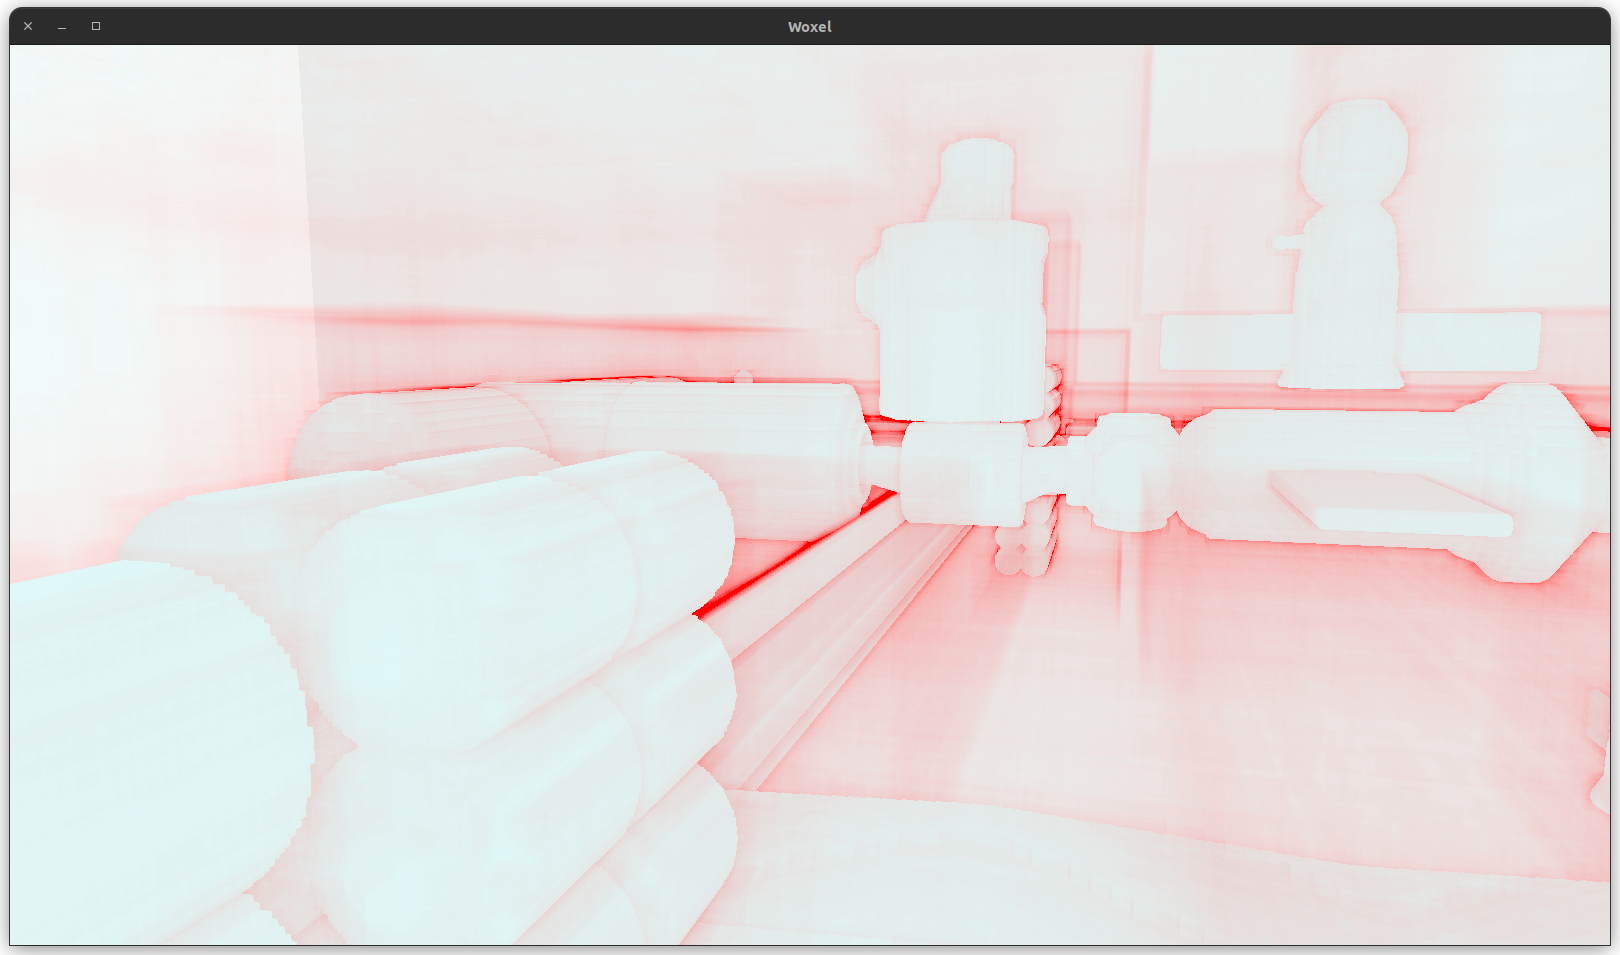
\includegraphics[width=\textwidth]{iss_sdf}
    \caption{}
  \end{subfigure}
  \caption[ISS HDDA vs. HDDA+SDF comparison]{Render in ray mode using (a) HDDA and (b) HDDA+SDF of the ISS model at position 3. The model resolution is $4561\times617\times2999$. The colour of pixels is determined analogously to \cref{teacomp}. The efficiency of the SDF method in high-detail areas can be clearly seen by comparing the two images: red patches in the middle of the image get much lighter, and bright red areas exist only very close to the model surface.}
\end{figure}

These two experiments prove the efficiency of the HDDA+SDF method; it gives more than 30 \% speedup over HDDA in all cases and is able to hit the frame rate cap of 165 FPS in most conditions. The high resolution of the test scenes used also proves that HDDA+SDF is a robust ray-marching algorithm that can handle complex scenes with good performance.

\subsection{Performance of HDDA+SDF in ray-tracing}

To test the performance of HDDA+SDF when ray-tracing, the average milliseconds per frame will be recorded in a number of scenes for both diffuse and glossy materials.

\begin{table}[h]
  \centering
  \begin{tabular}{|c||c|c|c|}
    \hline
    & bunny & dragon & ISS \\
    \hline
    diffuse & 6ms** & 6ms** & 6.5ms \\
    \hline
    glossy & 10.2ms & 11.6ms & 14ms \\
    \hline
  \end{tabular}
  \caption[Diffuse and glossy rendering times for bunny, dragon and ISS]{Milliseconds per frame to render each model with a diffuse and a glossy material. \\
    **: Frame rate cap is hit at 165 FPS; this is as good as the ray casting can get on this machine}
  \label{sdf_test}
\end{table}


\begin{figure}[H]
  \centering
  \begin{subfigure}[b]{0.32\textwidth}
    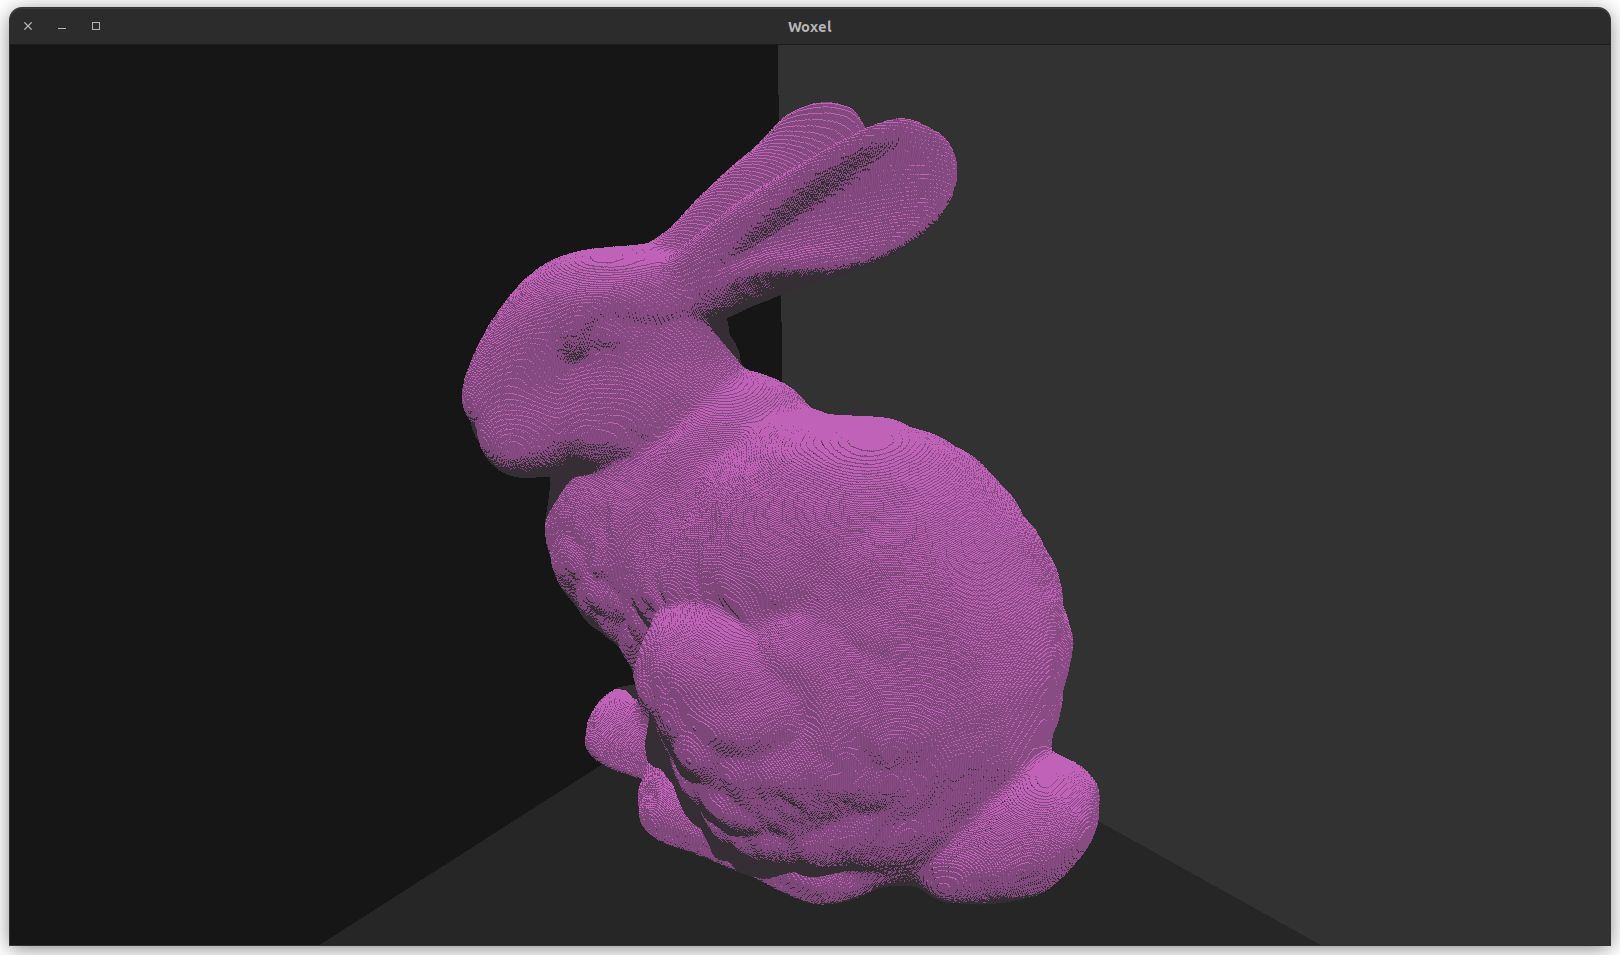
\includegraphics[width=\textwidth]{bunny_d}
    \caption{}
  \end{subfigure}
  \hfill
  \begin{subfigure}[b]{0.32\textwidth}
    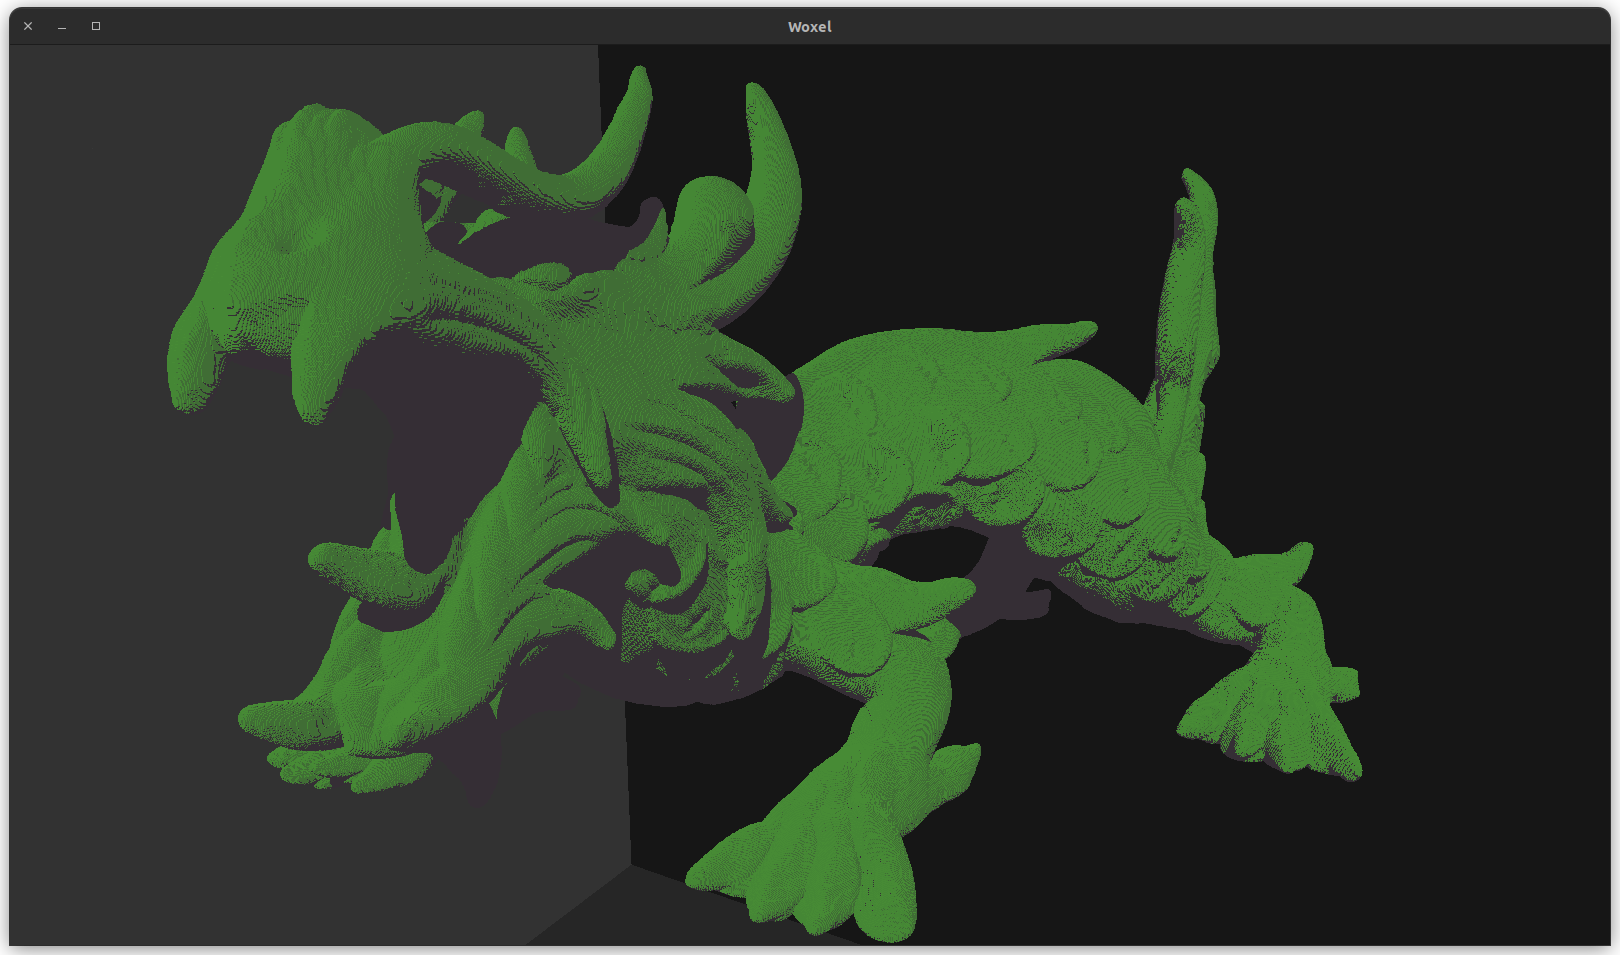
\includegraphics[width=\textwidth]{dragon_d}
    \caption{}
  \end{subfigure}
  \hfill
  \begin{subfigure}[b]{0.32\textwidth}
    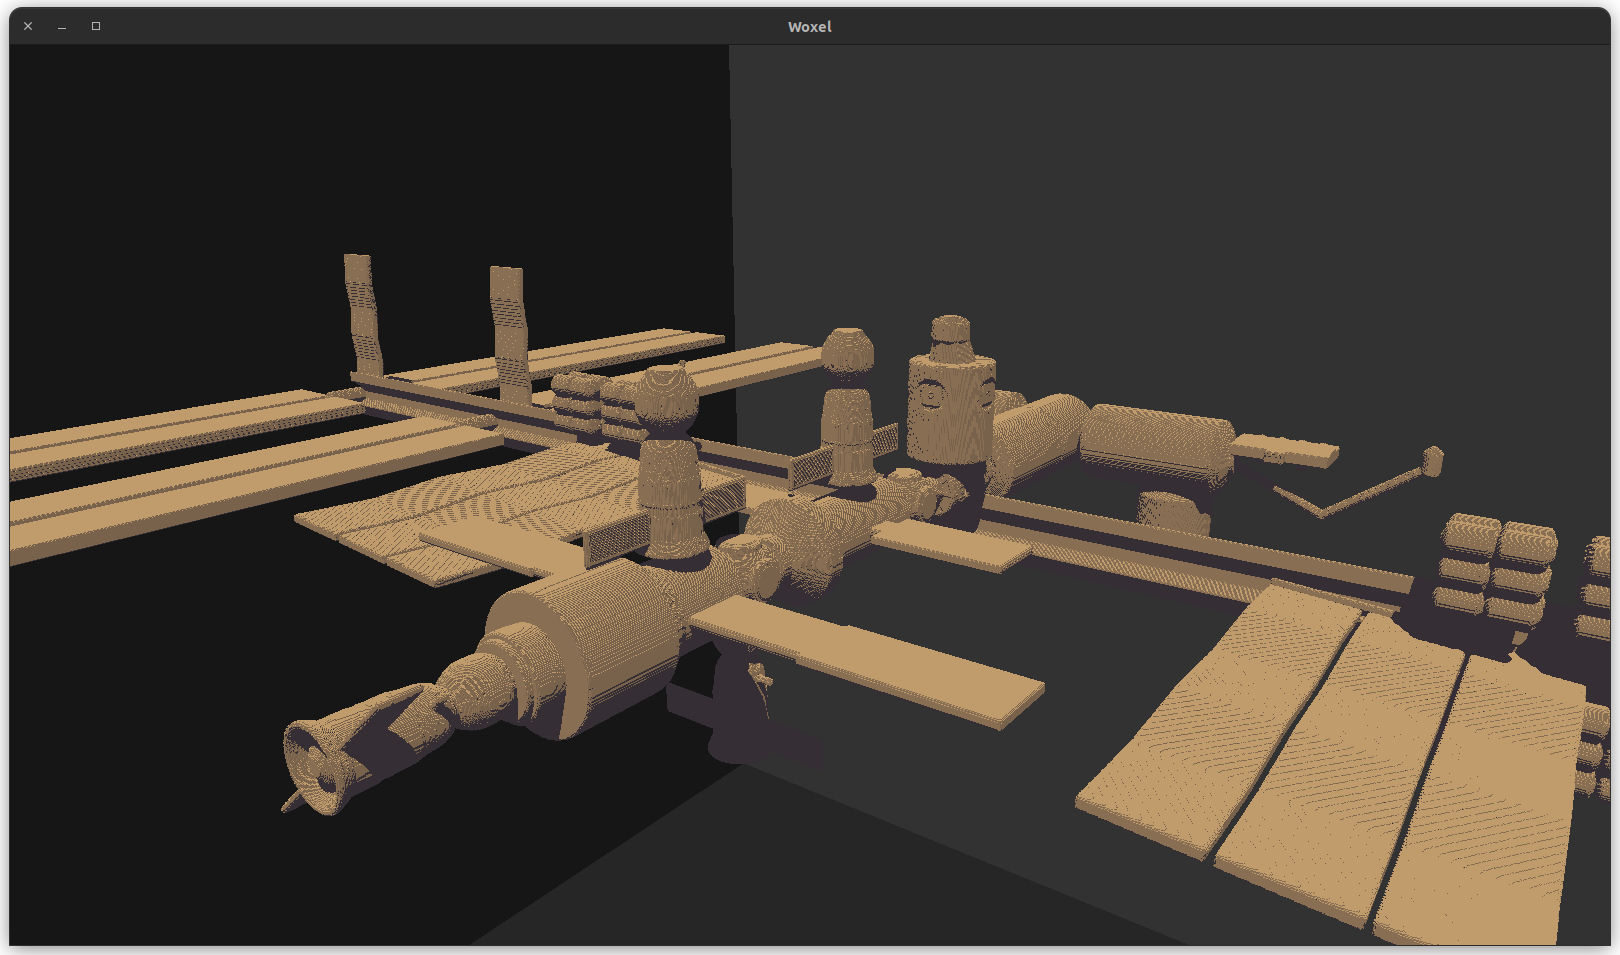
\includegraphics[width=\textwidth]{iss_d}
    \caption{}
  \end{subfigure}
  \hfill
  \begin{subfigure}[b]{0.32\textwidth}
    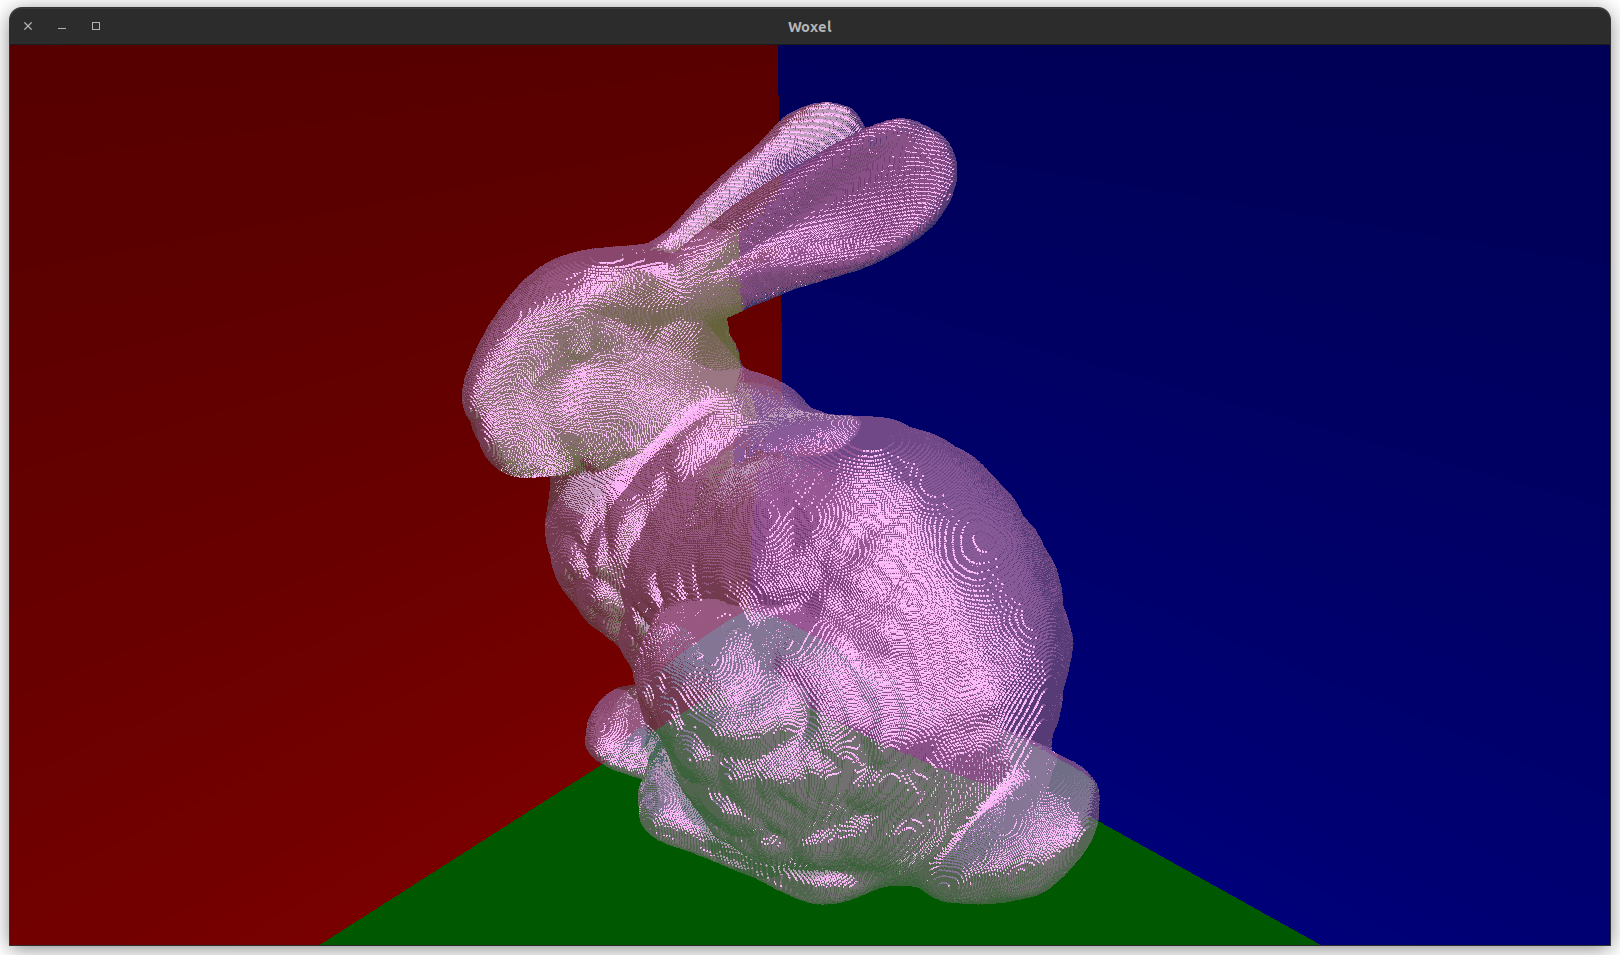
\includegraphics[width=\textwidth]{bunny_g}
    \caption{}
  \end{subfigure}
  \hfill
  \begin{subfigure}[b]{0.32\textwidth}
    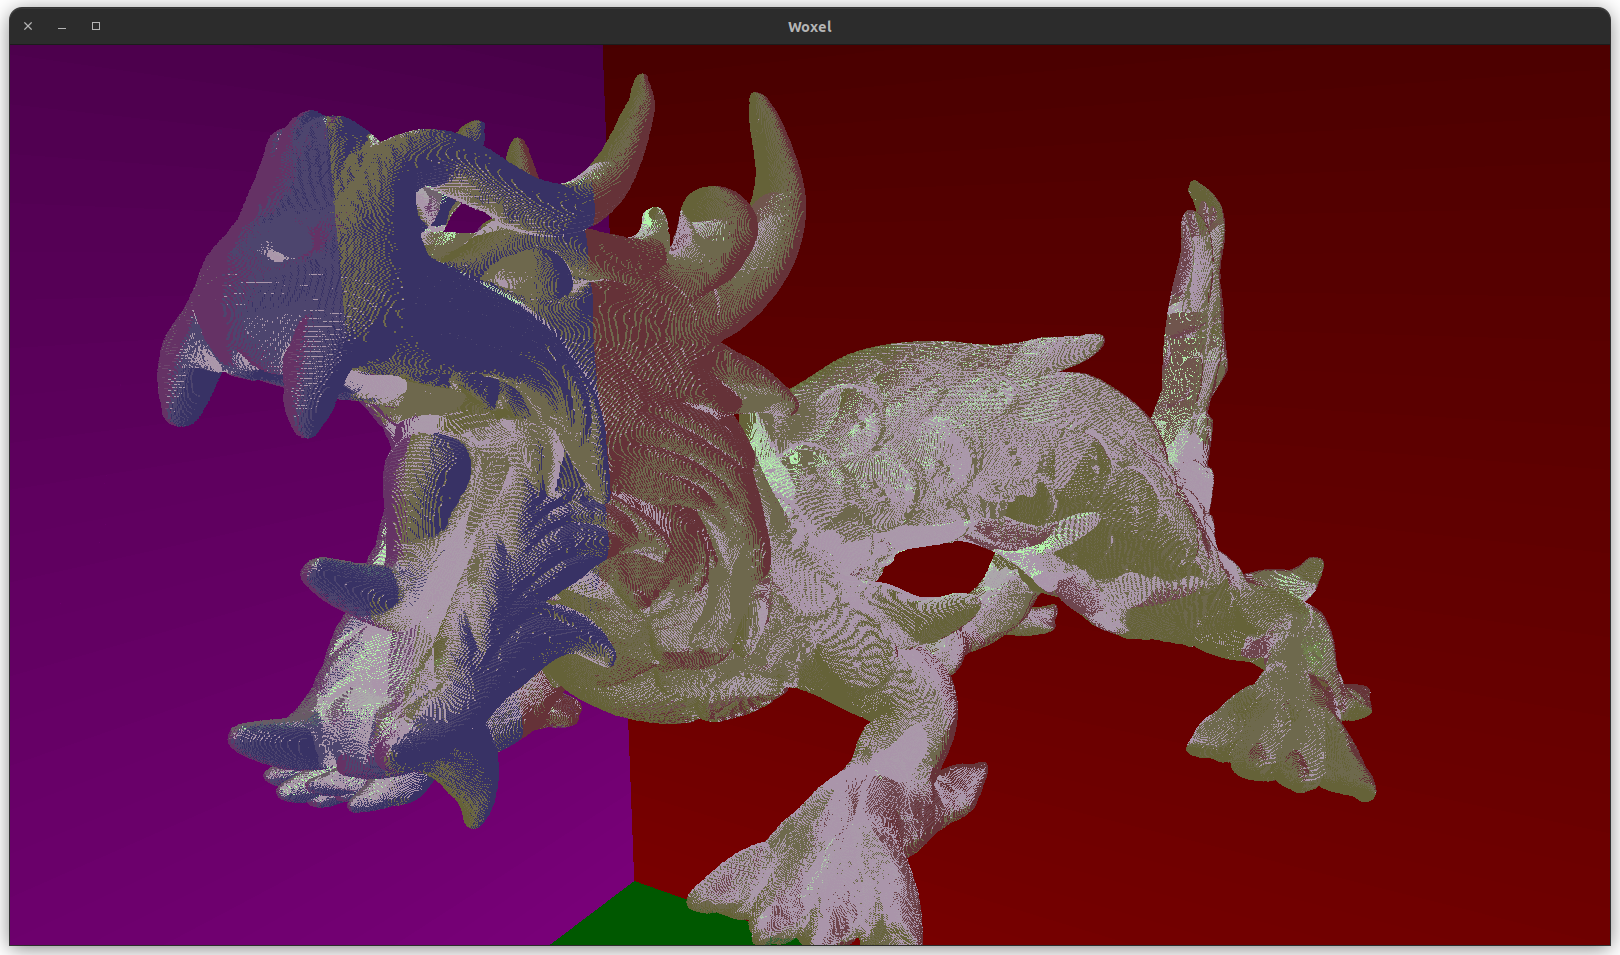
\includegraphics[width=\textwidth]{dragon_g}
    \caption{}
  \end{subfigure}
  \hfill
  \begin{subfigure}[b]{0.32\textwidth}
    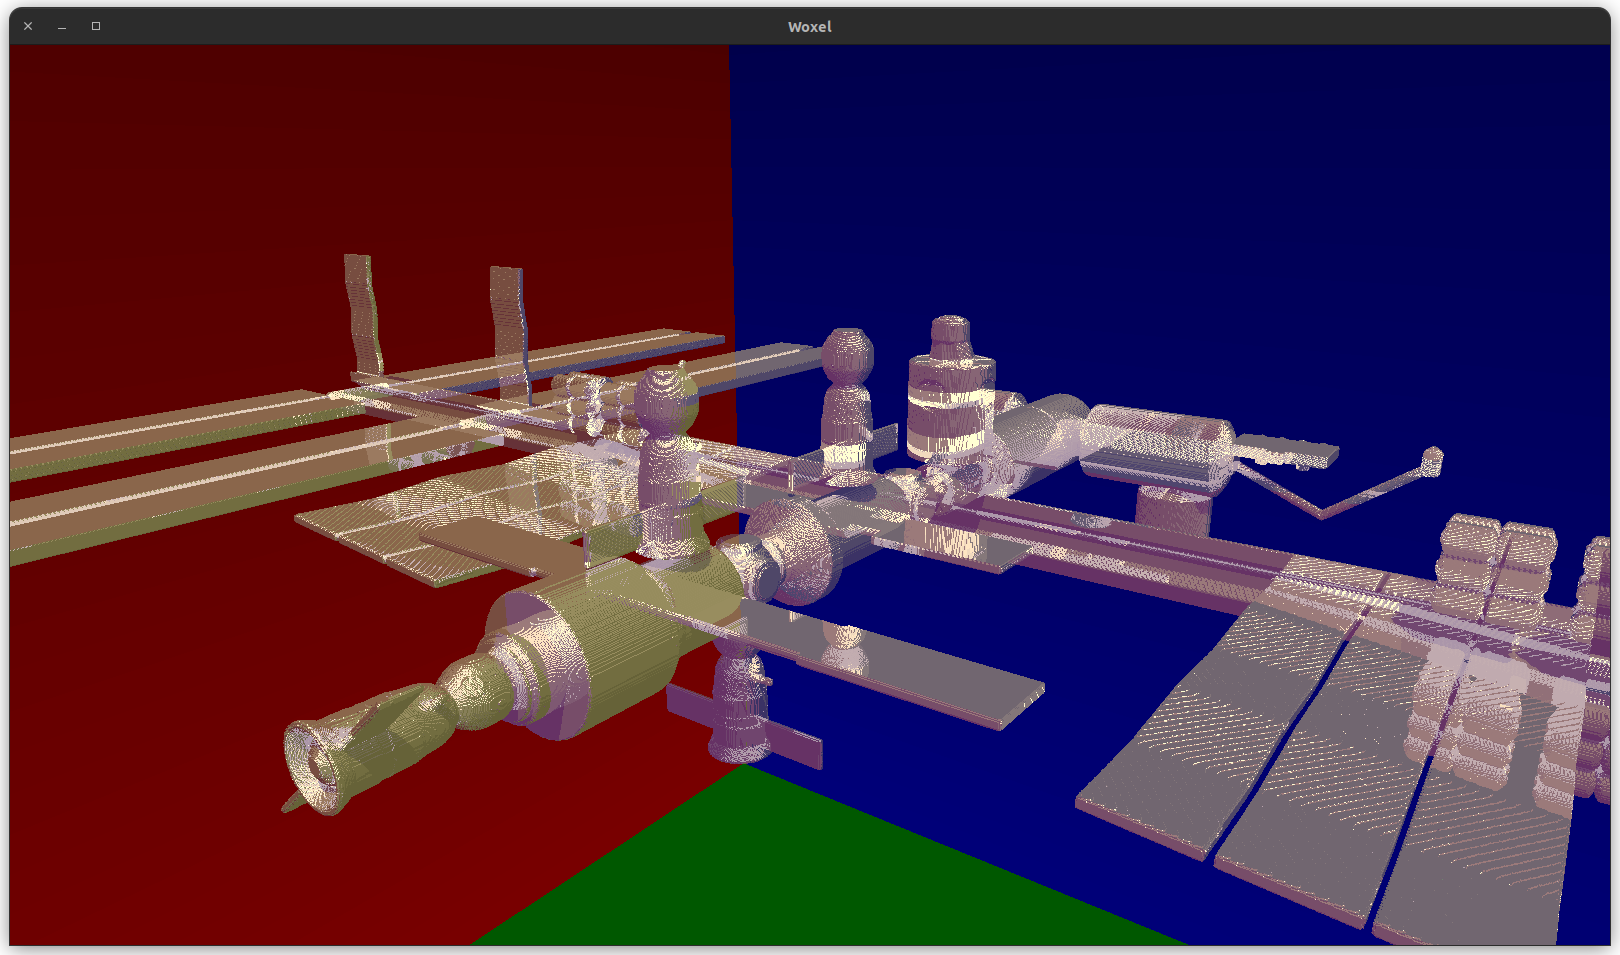
\includegraphics[width=\textwidth]{iss_g}
    \caption{}
  \end{subfigure}
  \caption[Diffuse and glossy renders]{Diffuse (a)-(c) and Glossy (d)-(f) renderings that produce the data int \cref{sdf_test}. (a) and (d) shows the bunny model, (b) and (e) shows the dragon model, (c) and (f) show the ISS model}
\end{figure}

The diffuse rendering scheme performs really well, with a minimum \acrshort{fps} of 150 on the large ISS model and capping out for the other two. The glossy material has a minimum FPS of 71 on the largest model, with each ray being allowed to be reflected twice. This produces reasonably looking glossy materials, but such a small maximum ray reflection count cannot produce photorealistic results. Scaling up the max ray reflection count is infeasible as the number of rays increases exponentially with it, and two is the maximum the engine can handle while staying above 60 FPS.

This shows that the HDDA+SDF performs very well with diffuse materials and dynamic lighting at over 150 FPS and that it is able to accommodate a small amount of reflections off glossy materials, all with around 80 FPS. This means this algorithm is a viable tool for real-time ray tracing.
